\chapter{The universal symmetry: the circle}
\label{cha:circle}

An effective principle in mathematics is that when you want to study a certain
phenomenon you should search for a single type that captures this phenomenon.
Here are two examples:\footnote{%
  Notice that these have arrows pointing in different directions:
  In~\cref{it:one-out} we're mapping \emph{out} of $\bn{1}$,
  while in~\cref{it:prop-in} we're mapping \emph{in} to $\Prop$.}
\begin{enumerate}
\item\label{it:one-out}
  The contractible type $\bn 1$ has the property that given
any type $A$ a function $\bn 1\to A$ provides exactly the
same information as picking an element in $A$.
For, an equivalence from $A$ to $\bn 1\to A$ is provided by
the function $a \mapsto (x \mapsto a)$.
\item\label{it:prop-in}
  The type $\Prop$ of propositions has the property that
given any type $A$ a function $A\to\Prop$ provides exactly
the same information as picking a subtype of $A$.
\end{enumerate}
We are interested in symmetries, and so we should search for a type $X$
which is so that given \emph{any} type $A$ the type of functions
$X\to A$ (or $A\to X$, but that's not what we're going to do)
picks out exactly the symmetries in $A$.
We will soon see that there is such a type:
the circle\footnote{%
  We call this type the ``circle''
  because it turns out to be the homotopy type of
  the topological circle $\setof{(x,y)\in\RR^2}{x^2+y^2=1}$.
  In the later chapters on geometry we'll return
  to ``real'' geometrical circles.}
which is built \emph{exactly} so that this
``universality with respect to symmetries'' holds.
It may be surprising to see how little it takes to define it;
especially in hindsight when we eventually discover some of the many uses of the circle.

A symmetry in $A$ is an identification $p:a=_Aa$ for some $a:A$.%
\index{symmetry!in a type}
Now, we can take any iteration of $p$ (composing $p$ with itself a number of times),
and we can consider the inverse $p^{-1}$ and \emph{its} iterations.
So, by giving one symmetry we at the same time give a lot of symmetries.
For a particular $p$ it may be that not all of the iterations are different,
for instance it may be that $p^2=p^0\defequi\refl a$ (like in \cref{xca:C2}),
or even more dramatic: if  $p=\refl a$, then \emph{all} the iterates of $p$ are equal.\marginnote{%
  \begin{tikzpicture}
    \node (A) at (0,-1.5) {$A$};
    \begin{scope}[thick]
      \draw (0,-1)
      .. controls ++(200:-1) and ++(180:1) .. (2,-2)
      .. controls ++(180:-1) and ++(270:1) .. (4,0)
      .. controls ++(270:-1) and ++(10:1)   .. (2,2.25)
      .. controls ++(10:-1)   and ++(90:1)  .. (-.5,1)
      .. controls ++(90:-1)  and ++(200:1) .. (0,-1);
      \pgfmathsetmacro\gsize{3}%
      \pgfmathsetmacro\gscale{min(1,\gsize/4)}%
      \pgfmathsetmacro\gyscale{0.25*\gscale*.707}%
      \pgfmathsetmacro\gxscale{0.5*\gscale}%
      \pgfmathsetmacro\gsep{((\gsize - 2*\gscale)/2*0.5)}%
      \pgfmathsetmacro\omrstwo{1 - 1/sqrt(2)}%
      \pgfmathsetmacro\sqrtwo{sqrt(2)}%
      \draw (1 + \gsep +  \gxscale + \gxscale -\omrstwo*\gxscale,0)
      .. controls +(-\gxscale*\sqrtwo/3,4/3*\gyscale)
      and +(\gxscale*\sqrtwo/3,4/3*\gyscale)
      .. ++(-\sqrtwo*\gxscale,0);
      \draw (1 + \gsep +  \gxscale - \gxscale,0 + \gyscale)%
      .. controls +(\gxscale*2/3,-8/3*\gyscale)
      and +(-\gxscale*2/3,-8/3*\gyscale)
      .. ++(2*\gxscale,0);
    \end{scope}
    \begin{scope}[shift={(-1.25,-7.25)}]
      \node[dot,label=right:$a$] (a) at (1.99,7.58) {};
      \draw[->]
      (4.02,7.58) .. controls (3.97,8.13) and (3.93,8.66) .. node[auto,swap] {$p$}
      (3.07,8.60) .. controls (2.20,8.54) and (1.99,8.00) ..
      (1.99,7.58) .. controls (1.98,7.15) and (2.25,6.67) ..
      (2.97,6.56) .. controls (3.70,6.44) and (4.06,7.03) ..
      (4.02,7.58);
      \draw[casblue,->]
      (3.25,6.44) .. controls (4.01,6.46) and (4.59,7.71) ..
      (3.77,8.45) .. controls (2.95,9.20) and (1.83,8.42) ..
      (1.81,7.60) .. controls (1.79,6.78) and (3.00,5.63) ..
      (3.94,6.67) .. controls (4.88,7.71) and (4.02,8.50) ..
      (3.54,8.78) .. controls (3.05,9.05) and (1.99,8.45) .. node[auto,swap] {$p^2$}
      (1.99,7.58) .. controls (1.99,6.70) and (2.49,6.42) ..
      (3.25,6.44);
      \draw[casred,->]
      (3.12,8.52) .. controls (3.69,8.49) and (3.81,8.27) ..
      (3.87,7.75) .. controls (3.93,7.23) and (3.67,6.58) ..
      (2.95,6.65) .. controls (2.23,6.71) and (1.98,7.01) ..
      (1.99,7.58) .. controls (2.00,8.14) and (2.55,8.55) ..
      node[auto,swap] {$p^{-1}$}
      (3.12,8.52);
    \end{scope}
  \end{tikzpicture}}
However, in general we must be prepared that all the powers of $p$
(positive, $0$ and negative) are distinct.
Hence, the circle must have a distinct symmetry for every integer.
We would have enjoyed defining the integers this way,
but being that ideological would be somewhat inefficient.
Hence we give a more hands-on approach defining the circle
and the integers separately. Thereafter we prove that the type of
symmetries in the circle is equivalent to the set of integers.

\section{The circle and its universal property}
\label{sec:S1}

Propositional truncation from \cref{sec:prop-trunc} was
the first \emph{higher inductive type}, that is, an inductive type
with constructors both for elements and for identifications,
we introduced.
The circle is another example of a higher inductive type,
see Chapter~6 of the HoTT book\footcite{hottbook} for more information.

\begin{definition}
  \label{def:circle}
The circle is a type $\Sc:\UU$ with an element (constructor) $\base : \Sc$ and
an identification (constructor) ${\Sloop}: \base=\base$. For convenience and
clarity the (higher) induction principle for $\Sc$ is explained
by first stating a recursion principle for $\Sc$.

Let $A$ be a type. In order to define a function $f:\Sc\to A$,
it suffices to give an element $a$ of $A$ together with an
identification $l$ of type $a=a$. The function $f$ defined
by this data satisfies $f(\base)\jdeq a$ and
the recursion principle provides an (unnamed) element of
$\ap{f}(\Sloop)=l$.

\begin{marginfigure}
  \noindent\begin{tikzpicture}
    \node (A) at (2,3) {$\sum_{x:\Sc}A(x)$};
    \node (Sc) at (2,0) {$\Sc$};
    \node (Sloop) at (.9,-.5) {$\Sloop$};
    \draw[->] (A) -- node[auto] {$\fst$} (Sc);
    \draw[->] (-90:1 and .3) arc (-90:270:1 and .3);
    \node[basedot] at (-1,0) {};
    % then: A top and bottom
    \coordinate[label=above left:$A(\base)$] (A-top-left) at (-1,2.7);
    \coordinate (A-bot-left) at (-1,0.9);
    \coordinate (A-top-front) at (0,2.4);
    \coordinate (A-bot-front) at (0,0.7);
    \coordinate (A-top-back) at (0,2.8);
    \coordinate (A-bot-back) at (0,1.3);
    \coordinate (A-top-right) at (1,2.6);
    \coordinate (A-bot-right) at (1,0.8);
    \draw (A-top-left) -- (A-bot-left)
    .. controls +(-90:.3) and +(-10:-.5) .. (A-bot-front)
    .. controls +(-10:.5) and +(90:-.3) .. (A-bot-right)
    -- (A-top-right)
    .. controls +(-90:.2) and +(170:-.5) .. (A-top-front)
    .. controls +(170:.5) and +(90:-.2) .. (A-top-left);
    \draw[dashed] (A-bot-left)
    .. controls +(90:.3) and +(5:-.4) .. (A-bot-back)
    .. controls +(5:.4) and +(-90:-.3) .. (A-bot-right);
    \draw (A-top-left)
    .. controls +(90:.3) and +(-10:-.3) .. (A-top-back)
    .. controls +(-10:.3) and +(-90:-.3) .. (A-top-right);
    \node[dot,label=left:$a$] (a-left) at (-1,2) {};
    \coordinate (a-front) at (0,1.6);
    \coordinate (a-right) at (1,1.8);
    \coordinate (a-back) at (0,2.2);
    \draw[->] (a-left)
    .. controls +(-90:.3) and +(-15:-.4) .. (a-front);
    \draw (a-front)
    .. controls +(-15:.4) and +(90:-.3) .. node[auto] {$l$} (a-right);
    \draw[dashed] (a-left)
    .. controls +(90:.3) and +(-5:-.4) .. (a-back)
    .. controls +(-5:.4) and +(-90:-.3) .. (a-right);
  \end{tikzpicture}
  \caption{The induction principle of $\Sc$.}
  \label{fig:circle-induction}
\end{marginfigure}

Let $A(x)$ be a type for every $x:\Sc$. The induction principle of $\Sc$
states that, in order to define an element of $A(x)$ for every element $x$ of $\Sc$,
it suffices to give an element $a$ of $A(\base)$ together with an
identification $l$ of type $\pathover{a}{A}{\Sloop}{a}$,
cf.~\cref{fig:circle-induction}.
The function $f$ defined by this data satisfies $f(\base)\jdeq a$ and
the induction principle provides an element of $\apd{f}(\Sloop)=l$.
\end{definition}

Giving $a$ as above is referred to as `the base case', and
giving $l$ as `the loop case'. Given this input data to define
a function $f$ will often be abbreviated by writing
$f(\base)\defeq a$ and $f(\Sloop)\defis l$.

The following result states that any function from the circle exactly
picks out an element and a symmetry of that element.
This is a ``universal property'' of the circle.

\begin{theorem}\label{lem:freeloopspace}
For all types $A$, the evaluation function
\[
\ev_A : (\Sc\to A)\to \sum_{a:A}(a=_Aa)\text{~defined by~}
\ev_A(g)\defeq (g(\base),g(\Sloop))
\]
is an equivalence, with inverse $\ve_A$ defined by the recursion principle.
\end{theorem}
\begin{proof}
Fix $A:\UU$. We apply \cref{lem:weq-iso}.
For all $a:A$ and $l:a=a$ we have $\ev(\ve(a,l))=(a,l)$
by the recursion principle. It remains to prove
$\ve(\ev(f))=f$ for all $f:\Sc\to A$. This will follow
from the following more general result.
Let $f,g:\Sc\to A$,
$p: f(\base)= g(\base)$, and $q: f(\Sloop) = p^{-1}\cdot g(\Sloop)\cdot p$.
We show $f=g$, for which it suffices to prove by circle induction
that $P(x)\defeq(f(x)=g(x))$ for all $x:\Sc$.
For the base case we take $p$.
The loop case reduces to $\trp[P]{\Sloop}(p)=p$ by \cref{def:pathover-trp}.
By \cref{lem:trp-in-fx=Ygx} we have
$\trp[P]{\Sloop}(p)=g(\Sloop)\cdot p \cdot f(\Sloop)^{-1}$.
By $q$ we have $g(\Sloop) = p\cdot f(\Sloop) \cdot p^{-1}$.
Hence $\trp[P]{\Sloop}(p)=p$ by easy calculation.
Using \cref{lem:isEq-pair=} we can phrase the result
as: if $\ev(f)=\ev(g)$, then  $f=g$.

Now we get $\ve(\ev(f))=f$, as
$\ev(\ve(\ev(f)))=(f(\base),f(\Sloop))\jdeq\ev(f)$ with $p\defeq\refl{f(\base)}$
and $q$ coming from the induction principle.
\end{proof}
\begin{corollary}\label{cor:circle-loopspace}
  For any $a:A$, the function $\ev_A^a:((\Sc,\base)\to_* (A,a))\to (a=_Aa)$
  sending $(g,p)$ to $p^{-1}\cdot g(\Sloop)\cdot p$ is an equivalence.
\end{corollary}
\begin{proof}\hskip-5pt\footnote{%
    This can also be done directly:
    The inverse to $\ev_A^a$ sends $l : a=_Aa$
    to $(\ve_A(a,l), \refl{a})$.
    Try to verify this!}
It's easy to check commutativity of the diagram
\[
  \begin{tikzcd}
    (\Sc \to A) \ar[rr,"{g\mapsto(g(\base),g,\refl{g(\base)})}"]
    \ar[dr,"\ev_A"'] & &
    \sum_{a:A}\bigl((\Sc,\base) \ptdto (A,a)\bigr)
    \ar[dl,"\tot(\ev_A^-)"] \\
    &  \,\sum_{a:A}(a=_A a),
  \end{tikzcd}
\]
where the top map is an equivalence by \cref{cor:contract-away},
and the left map is an equivalence by \cref{lem:freeloopspace}.
The result now follows from \cref{lem:fiberwise-equiv-from-tot}.
\end{proof}

\begin{remark}\label{rem:dep-univ-prop-circle}
By almost the same argument as for \cref{lem:freeloopspace}
one can obtain the dependent universal property of the circle.
Given a type family $A:\Sc\to\UU$, the evaluation function
$(\prod_{x:\Sc} A(x))\to \sum_{a:A(\base)}(\pathover a A {\Sloop} a)$
is an equivalence.
\end{remark}

\begin{marginfigure}
  \begin{tikzpicture}
    %% draw S1
    \node[dot,label=below:$\Sc$] (base) at (0,0) {};%
    \draw[->] (base) .. controls ++(45:1) and ++(135:1) .. node (loop)
    {} (base);
    %% type A
    \begin{scope}[xshift=5em]
      \draw plot [smooth cycle] coordinates {(0,0) (1.5,0) (1.3,1)
        (0,1.5)};%
      \node[dot,label=below:$a$] (a) at (.5,.5) {};%
      \node (A1) at (1.5,1.5) {$A$}; \draw[->] (a) .. controls
      ++(-20:1) and ++(-30:.5) .. ++(45:.5) .. controls ++(150:1) and
      ++(210:1) .. node[very near start] (middle) {} (a);
    \end{scope}
    %% draw map f
    \draw[dashed, ->, shorten <= 3pt, shorten >= 3pt] (loop) to[bend
    left] node[above]{$f$} (middle);
  \end{tikzpicture}
\end{marginfigure}
\begin{remark}
  A function $f:\Sc\to A$ is often called a \emph{loop} in $A$, the
  picture being that $f$ throws $\Sloop:\base=\base$ as a lasso in the
  type $A$.

  Using the above equivalence, so that $a=_Aa$ is identified with the pointed
  functions from the circle, this allows for a very graphic
  interpretation of the symmetries of $a$ in $A$: they are traced out
  by a function $f$ from the circle and can be seen as loops in the type
  $A$ starting and ending at $a$!\footnote{%
    This is of course how we have been
    picturing loops the whole time.}
\end{remark}

\begin{lemma}\label{lem:circleisconnected}
  The circle is connected.
\end{lemma}
\begin{proof}
We show $\Trunc{\base=z}$ for all $z:\Sc$ by circle induction
as in \cref{def:circle}.
For the base case we take $\trunc{\refl{\base}}$.
The loop case is immediate as $\Trunc{\base=\base}$ is a proposition.
\end{proof}

In the proof above, the propositional truncation coming
from the definition of connectedness is essential.
If this truncation were removed we wouldn't know what to do in
the induction step (actually, ${\base=z}$ for all $z:\Sc$ contradicts UA).
This said, the family $R:\Sc\to\UU$ with $R(z)\defequi (\base=z)$ is extremely
important for other purposes. We will call it in \cref{def:universalcover} the
``universal \covering'' of the circle and it is the key tool in proving that
the set of integers and the symmetries in the circle can be identified.
Recall that we
use the phrase ``symmetries \emph{in} the circle'' to refer to the
elements of $\base=_{\Sc}\base$,\footnote{%
  Here we are using ``the circle'' to mean the
  \emph{pointed} type $(\Sc,\base)$.
  But it also turns out that the type $\base=_{\Sc}\base$ is
  equivalent to the type $x=_{\Sc}x$, for any $x:\Sc$.}
whereas we use the phrase ``symmetries \emph{of} the circle'' to refer to the elements of $\Sc=_{\UU}\Sc$.
The latter type is equivalent to $\Sc\amalg\Sc$,
as follows from \cref{xca:S1=S1-components} and \cref{{xca:(S1->S1)_(f)-eqv-S1}}.

In order to proceed, we should properly define the set of integers
and explore the concept of \coverings.

\section{The integers}
\label{sec:integers}

We define the type of integers in one of the many possible ways.\footnote{%
  Here are some of these alternatives:
  \begin{itemize}
  \item As the copy of $\NN$ where $2n$ means $n$ and $2n+1$ means $-n-1$, for $n:\NN$.
  \item As the sum $\NN\coprod\NN$, where $\inl{n}$ means $-n-1$ and $\inr{n}$ means $n$.
  \item As the sum $\NN\coprod\bn1\coprod\NN$, where from the left copy of $\NN$ we get $-n-1$, from the center $0:\bn1$ we get $0$, and from the right copy of $\NN$ we get $n+1$, for $n:\NN$.
  \item As the quotient of $\NN\times\NN$ under the equivalence relation
    $(n,m) \sim (n',m')$ defined by $n+m' = n'+m$,
    where $(n,m)$ represents $n-m$.
  \item As the subset of $\NN\times\NN$ consisting of those $(n,m)$ with $n=0\lor m=0$ (picking canonical representatives for the above equivalence relation).
  \item As the loops $\base=_\Sc\base$ in the circle. %$\ddot\smile$
  \end{itemize}}

\begin{definition}\label{def:zet}
  Let $\zet$ be the higher inductive type with the following three
  constructors:\glossary(Z){$\protect\zet$}{the set of integers,
  \cref{def:zet}}
\begin{enumerate}
\item $\iota_+: \NN \to \zet$ for the nonnegative numbers,
  $0,1,\ldots$\glossary(909iota+){$\iota_+$}{embedding of $\NN$ into $\zet$}
\item $\iota_-: \NNN \to \zet$ for the nonpositive numbers,
  $-0,-1,\ldots$\glossary(909iota-){$\iota_-$}{embedding of $\NNN$ into $\zet$}
\item $\zeq : \iota_-(-0) = \iota_+(0)$.
\end{enumerate}
Because we used the copy $\NNN$ for the nonpositive numbers from \cref{exa:nnn},
we can leave out the constructor symbols $\iota_\pm$
when the type is clear from context.
Thus we have $\ldots,-2,-1,-0,0,1,2,\ldots:\zet$ and $\zeq:-0=_\zet0$.

The type $\zet$ comes with an induction principle:
Let $T(z)$ be a family of types indexed by $z:\zet$.
In order to construct an element $f(z)$ of $T(z)$ for all $z:\zet$,
it suffices to give functions $g$ and $h$ such
that $g(n): T(\iota_+(n))$ and $h(n): T(\iota_-(m))$ for all $n:\NN,m:\NNN$,
together with $q : \pathover {h(-0)} T \zeq {g(0)}$.
Here $g$ and $h$ can be defined by induction on $n:\NN,m:\NNN$.\footnote{%
  Of course, giving $h$ is the same as giving $h':\prod_{n:\NN}T(-n)$.}

The resulting function $f:\prod_{z:\zet}T(z)$ satisfies
$f(n)\jdeq g(n)$ and $f(-n)\jdeq h(-n)$ for $n:\NN$,
and there is an (unnamed) element of $\apd{f}(\zeq) = q$.
\end{definition}

Like the type $\NN$, the type $\zet$ is a set with decidable equality
and ordering relations.

One well-known self-equivalence is \emph{negation}, ${-}:\zet\to\zet$,
also called \emph{complement}, inductively defined by setting
$-\iota_+(n)\defeq \iota_-(-n)$,
$-\iota_-(m)\defeq \iota_+(-m)$,
$\constant{ap}_-(\zeq) \defis \inv{\zeq}$.\footnote{%
  Here we included the constructor symbols for clarity,
  but the definition allows us to use the negation symbol
  unadorned, because the following diagram
  commutes (even up to definitional equality):
  \[
    \begin{tikzcd}[column sep=large,row sep=large,ampersand replacement=\&]
      \NN \ar[r,shift left=1mm,"-"]\ar[d,"\iota_+"']
      \& \NNN \ar[l,shift left=1mm,"-"]\ar[d,"\iota_-"] \\
      \zet \ar[r,shift left=1mm,"-"]
      \& \zet \ar[l,shift left=1mm,"-"]
    \end{tikzcd}
  \]}
Negation is its own inverse.

The \emph{successor} function $\zs:\zet\to\zet$%
\glossary(s){$\protect\zs$}{successor function on $\zet$} is
likewise defined inductively, setting
$\zs(n) \defeq \Succ(n)$,
$\zs(-0) \defeq 1$,
$\zs(-\Succ(n)) \defeq -n$,
and $\ap{\zs}(\zeq) \defis \refl{1}$.

The successor function $\zs$ is an equivalence.
It is instructive to depict iterating $\zs$ in both directions as
a doubly infinite sequence containing all integers:
\[
  \begin{tikzcd}[arrows=mapsto,row sep=tiny]
    & & & -0 \ar[dd,eqr]\ar[dr] & & & \\
    \cdots\ar[r] & -2\ar[r] & -1\ar[ur] & & 1\ar[r] & 2\ar[r] & \cdots \\
    & & & 0 \ar[ur] & & &
  \end{tikzcd}
\]

The inverse $\inv\zs$ of $\zs$ is called the \emph{predecessor} function.
We recall the $n$-fold iteration $\zs^n$ defined earlier;
the $n$-fold iteration of $\zs^{-1}$ will be denoted by $\zs^{-n}$.
Since $\zs^0 \jdeq \id \jdeq \zs^{-0}$,
this defines the iteration $\zs^z$ for all $z:\zet$.\footnote{%
  In the same way, we can define the iteration
$f^z : X \to X$ for any \emph{equivalence} $f : X \to X$.}\index{iteration}

\emph{Addition} of integers is now defined by iteration:
$z + y \defeq \zs^{y}(z)$.
This extends $+$ on the $\iota_+$-image of $\NN$,
see \cref{xca:addition-on-Z-and-N}.
From addition and unary $-$ one can define a binary
\emph{subtraction} function setting $z-y \defeq z+(-y)$.
Since addition and subtraction are mutually inverse,
we may iterate addition to define \emph{multiplication}:
$zy \defeq (w \mapsto w+z)^y(0)$.

\begin{xca}\label{xca:addition-on-Z-and-N}
  Show that $\iota_+(n+m)=\iota_+(n)+\iota_+(m)$
  and $\iota_+(nm) =\iota_+(n)\iota_+(m)$ for all $n,m:\NN$.
\end{xca}

The ordering relations $<$ and $\leq$ on $\zet$ are easily defined
and shown to extend those on $\NN$.

Recall the induction principle for $\zet$ in \cref{def:zet} above.
Instead of defining $g$ and $h$ explicitly, we will often
give $f(0)$ directly, and
define $g'$ and $h'$ such that $g'(z): T(z)\to T(z+1)$
for all $z:\zet$ with $z\geq 0$, and $h'(z): T(z)\to T(z-1)$
for all $z:\zet$ with $z\leq 0$. The function $f$ thus defined
satisfies $f(-0) \jdeq f(0)$,
$f(z+1)\jdeq g'(z,f(z))$ for all $z\geq 0$,
and $f(z-1)\jdeq h'(z,f(z))$ for all $z\leq 0$.

\begin{xca}\label{xca:commutative-add-Z}
  Show that $x+y = y+x$ and $xy=yx$ for all $x,y:\zet$.
\end{xca}

\section{\Coverings}
\label{sec:covering}

As mentioned earlier, it is possible to define the integers as the
type $\base=_{\Sc}\base$ of symmetries in the circle.
Our investigation of $\base=_{\Sc}\base$ will use the concept of \coverings.
Since we are going to return to this concept several times,
we take the time for a fuller treatment before we continue with
proving the equivalence of $\base=_{\Sc}\base$ and $\zet$.

\begin{definition}\label{def:covering}
A \emph{\covering} over a type $B$
is a map $f:A\to B$ such that for each $b:B$ the preimage $f^{-1}(b)$ is a set.
We say that a \covering $f:A\to B$ over $B$ is
\begin{itemize}
\item \emph{connected}\index{connected \covering} if $A$ is connected,
\item \emph{universal}\index{universal \covering} if $A$ and all
the identity types $a=_Aa$ (for $a:A$) are connected,
\item \emph{finite}\index{finite \covering} if all preimages are finite sets,
\item \emph{decidable}\index{decidable \covering} if all preimages are decidable sets.
\end{itemize}
If $B$ is a pointed type, a \emph{pointed} \covering is a pointed map $f:A\to_*B$ such that, when forgetting the points, $f_\div:A_\div\to B_\div$ is a \covering. Here we only
require $A$ to be a pointed type.\footnote{%
  If we forget the base point of $B$, and the pointedness of $f$, $f_0$,
  then these can be recovered uniquely, by setting $\pt_B \defeq f(\pt_A)$
  and $f_0 \defeq \refl{\pt_B} : \pt_B = f(\pt_A)$.
  Indeed, the forgetful map $\Bigl(\sum_{b:B}(A,a)\ptdto(B,b)\Bigr)
  \to (A \to B)$ is an equivalence by \cref{cor:contract-away}.}
We do not require the preimages of $f_\div$ to be pointed types.
\end{definition}
With a formula, given a type $B$, the type of \coverings over $B$ is
\[
\SetBundle(B) \defeq \sum_{A:\UU}\sum_{f:A\to B}\prod_{b:B}\isset(f^{-1}(b)),
\]
with variations according to the flavor.

Recall the equivalence in \cref{lem:Prop-Set-pointed-families}\ref{lem:Set-families}
between the type $B\to\Set$ of families of sets indexed by $B$, and the type
of \coverings over $B$ given above.
We shall frequently use this equivalence, even without explicit mention.

\begin{lemma}\label{lem:setbundle-is-groupoid}
For any type $B$, $\SetBundle(B)$ is a groupoid.
\end{lemma}
\begin{proof}
By \cref{lem:Set-is-groupoid} we have that $\Set$ is a groupoid,
and hence $B\to\Set$ is a groupoid by \cref{lem:level-n-utils}\ref{level-n-utils-codom}.
Moreover, by \cref{cor:subtype-same-level}, all variations in \cref{def:covering}
defined by a predicate are groupoids as well.
\end{proof}
One notable exception to the above lemma is the type of \emph{pointed} \coverings:
a point is extra structure, not just a property.

We should notice that the notion of a \covering is just one step up from the notion of an
injection (a map such that all the preimages are propositions --
following the logic, injections perhaps ought to be called ``proposition bundles'').
The formulation we give is not the only one and for some purposes a formulation
based on $B\to\Set$ is more convenient.

\begin{xca}\label{xca:constant-cover}
Let $A,B$ and $C$ be types. Show:
\begin{enumerate}
\item The (unique) map of type $A\to\bn 1$ is a \covering iff $A$ is a set;
\item For any $b:B$, the map $x \mapsto b$ from $\bn 1$ to $B$ is
a \covering iff $b=b$ is a set;
\item If $f: A\to B$ and $g: B\to C$ are \coverings, then $gf$ is a \covering.\endproof
\end{enumerate}
\end{xca}

Figure~\ref{fig:covering} visualizes two examples of \coverings over the circle.
Consider the picture on the left first.
If we let $b$ be the element on the circle marked at the bottom left hand side,
then the preimage $f^{-1}(b)$ is marked by the the two dots in $A$ straight above $b$,
so that in this case each preimage contains two points (is \emph{merely equal} to $\bn 2$).
However, $A$ is not the constant family, like $A'$ depicted on the right, since
$A'=\sum_{z:\Sc}\bn 2=\Sc\times\bn 2=\Sc+\Sc$ is not connected.
Obviously something way more fascinating is going on.
(In fact the \covering on the left is given by $\ve_\UU(\bool,\twist)$,
see \cref{xca:C2} and \cref{lem:freeloopspace}.)

\begin{figure}[hbt]
  \begin{sidecaption}%
    {A visualization of two \coverings over the circle}[fig:covering]
  \centering
  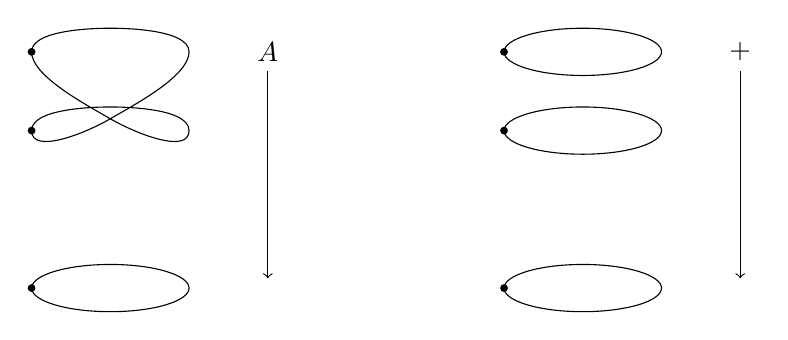
\begin{tikzpicture}
    \node (A) at (2,1) {$A$};
    \node (B) at (2,-2) {$\Sc$};
    \draw[->] (A) -- (B);
    \draw (0,-2) ellipse (1 and .3);
    \draw (-1,0)
    .. controls ++( 90:-.3) and ++(210: .4) .. (0,0.15)
    .. controls ++(210:-.4) and ++(270: .3) .. (1,1)
    .. controls ++(270:-.3) and ++(  0: .1) .. (0,1.3)
    .. controls ++(  0:-.1) and ++( 90: .3) .. (-1,1)
    .. controls ++( 90:-.3) and ++(150: .4) .. (0,0.15)
    .. controls ++(150:-.4) and ++(270: .3) .. (1,0)
    .. controls ++(270:-.3) and ++(  0: .1) .. (0,0.3)
    .. controls ++(  0:-.1) and ++( 90: .3) .. (-1,0);
    \node[fill,circle,inner sep=1pt] at (-1,-2) {};
    \node[fill,circle,inner sep=1pt] at (-1,0) {};
    \node[fill,circle,inner sep=1pt] at (-1,1) {};
%    \node (L) at (1,-3) {(left)};
    \begin{scope}[xshift=6cm]
    \node (At) at (2,1) {$\Sc+\Sc$};
    \node (Bt) at (2,-2) {$\Sc$};
    \draw[->] (At) -- (Bt);
    \draw (0,-2) ellipse (1 and .3);
    \draw (0,0) ellipse (1 and .3);
    \draw (0,1) ellipse (1 and .3);
    \node[fill,circle,inner sep=1pt] at (-1,-2) {};
    \node[fill,circle,inner sep=1pt] at (-1,0) {};
    \node[fill,circle,inner sep=1pt] at (-1,1) {};
%    \node (Lt) at (1,-3) {(right)};
    \end{scope}
  \end{tikzpicture}
  \end{sidecaption}
\end{figure}

\begin{remark}
  It \emph{is} possible to misunderstand what a ``connected \covering'' is:
the other interpretation ``all the preimages are connected''
would simply give us an equivalence (since connected sets are contractible),
and this is \emph{not} what is intended. (Equivalences are \coverings,
but not necessarily connected \coverings and connected \coverings are not neccesarily equivalences.)

Likewise for the other qualifications; for instance, in a ``finite covering'' $f:A\to B$,
the type $A$ is usually \emph{not} a finite set.

We trust the reader to keep our definitions in mind and not the other interpretations.
\end{remark}


\begin{remark}
  \Coverings are closely related to a concept from topology called ``covering spaces''
(or any variant of this concept, including Galois theory) and from algebra as locally constant sheaves (of sets).
Either way, the concept is useful because it singles out the (sub)symmetries.
\end{remark}

In this chapter, we focus on \coverings over the circle.

\begin{theorem}\label{thm:coveringsofS1perms}
  The evaluation function provides an equivalence
  \[
    \ev_\Set : (\Sc \to \Set) \to \sum_{X:\Set}(X=X)
    \quad\text{defined by $\ev_\Set(E) \defeq (E(\base),E(\Sloop))$.}
  \]
  Consequently, we have a string of equivalences
  \begin{align*}
    \SetBundle(\Sc)
    &\equiv (\Sc \to \Set)
      \equiv \sum_{X:\Set}(X=X) \\
    &\equiv \sum_{X:\Set}(X\equiv X)
    \equiv \sum_{X:\UU}\sum_{f:X\to X}
    \isset(X) \times \isEq(f).
  \end{align*}
\end{theorem}
\begin{proof}
  The first part is the universal property of the circle,
  \cref{lem:freeloopspace}, applied to $A\defeq\Set$.
  The equivalences then follow from \cref{lem:Prop-Set-pointed-families}\ref{lem:Set-families} and UA,
  together with minor manipulations.
\end{proof}
In slogan form: A \covering over the circle is a set with a permutation of its elements.
The fiber over $\base:\Sc$ gives the set,
and transporting along $\Sloop$ gives the permutation.

A particularly important example is the following:
\begin{definition}\label{def:RtoS1}
  The \covering $R:\Sc\to\UU$ corresponds to the integers with the successor operation.
  We have $R(\base)\defeq\zet$ and $R(\Sloop)\defis \etop{\zs}$.
  (This is indeed a set bundle since $\Sc$ is connected,
  so that $R(x)$ is a set for all $x:\Sc$.
  Abusing notation we also write $R:\Sc\to\Set$.)
  Now define
  \[
    \tilde R\defeq\sum_{z:\Sc}R(z)
  \]
  and let the first projection denoted by
  \[
    \exp:\tilde R \to \Sc
  \]
  be the \emph{exponential \covering of the circle}.
\end{definition}

\begin{remark} \label{rem:expforreal}%
  \begin{marginfigure}
    \begin{tikzpicture}[scale=.15]
      \node (Sc) at (0,-5) {$\Sc$};
      \node[dot,label=left:$2$]  (B)    at (-10,18) {};
      \node[dot,label=left:$1$]  (one)  at (-10,14) {};
      \node[dot,label=left:$0$]  (zero) at (-10,10) {};
      \node[dot,label=left:$-1$] (mone) at (-10, 6) {};
      \node[dot,label=left:$-2$] (C)    at (-10, 2) {};
      \node[dot]                 (D)    at (-10,-5) {};
      \node[label=above:$\tilde R$]   (R)    at (10,20) {};
      \node[label=above left:$\zet$]  (Z)    at (-10,20) {};
      \node at (-10,20.8) {$\vdots$};
      \node at (-10,.2) {$\vdots$};
      \node[label=left:$\Sloop$] (Sloop) at (10,-5) {};

      \pgfmathsetmacro\cc{.55228475}% = 4/3*tan(pi/8)
      \pgfmathsetmacro\cy{2*\cc}%
      \pgfmathsetmacro\cx{10*\cc}%
      \pgfmathsetmacro\ay{.35165954}%

      \draw (10,0) \foreach \y in {0,4,...,16} {
        .. controls (10,\y + \cy + \ay) and (\cx,3 + \y - \ay)
        .. (0,3 + \y) .. controls (-\cx,3 + \y + \ay) and (-10,2 + \y + \cy - \ay)
        .. (-10,2 + \y) .. controls (-10,2 + \y - \cy + \ay) and (-\cx,1 + \y - \ay)
        .. (0,1 + \y) .. controls (\cx,1 + \y + \ay) and (10,4 + \y - \cy - \ay)
        .. (10,4 + \y) } ;
      \draw (10,-5) .. controls (10,-5 + \cy) and (\cx,-3)
      .. (0,-3) .. controls (-\cx,-3) and (-10,-5 + \cy)
      .. (-10,-5) .. controls (-10,-5 - \cy) and (-\cx,-7)
      .. (0,-7) .. controls (\cx,-7) and (10,-5 - \cy) .. (10,-5);
    \end{tikzpicture}
  \end{marginfigure}
  The reason for the name ``exponential'' comes from the following
  visualization.  If $x$ is a real number, then the complex
  exponentiation $\ee^{2\pi\ii x}=\cos(2\pi x)+\ii\sin(2\pi x)$ has
  absolute value $1$ and so defines a continuous function from the
  real numbers to the unit circle.  Choosing any point $z$ on the unit
  circle, we see that the preimage of $z$ under the exponential
  function is a shifted copy of the integers inside the reals.\footnote{%
    Again, we emphasize that we are here dealing with the
    \emph{homotopy types} of the reals $\RR$ and the unit circle,
    $\setof{(x,y):\RR^2}{x^2+y^2=1}$.}

  This connection between the integers and the unit circle is
  precisely captured in a form that we can take further by studying the
  \covering $\exp:\tilde R\to \Sc$.
\end{remark}

We already defined a \covering $f:A\to B$ to be universal if $A$ is connected
and all $a=_A a$ (for $a:A$) are connected.
If moreover $B$ is a pointed, connected groupoid we shall argue that
we actually can speak of \emph{the} universal \covering.

Recall \cref{cor:fib-vs-path} stating that all the fibers of a map $f:A\to B$
are sets if and only if each
\[
\ap{f}: (a=a')\to (f(a)=f(a'))
\]
is an injection.
Assume $f:A\to B$ is a universal \covering and $B$ is a groupoid.
We prove that $A$ is contractible.
Being contractible is a proposition, so we may assume
we have an element $a$ of $A$ since $A$ is connected.
By \cref{xca:connected-trivia} and \ref{xca:component-connected}
it suffices to prove that $a=a$ is contractible.
By \cref{xca:prop-set-trivia}, using that $a=a$ is connected,
it suffices to show that $a=a$ is a set.
Using that $\ap{f}$ is an injection, we can apply the remark after
\cref{lem:sum-of-fibers} and obtain that $a=a$ is a set since
$f(a)=f(a)$ is a set, since $B$ is a groupoid.
This completes the proof that $A$ is contractible.

Now assume $(B,b_0)$ is a pointed connected groupoid and $f:A\to B$
a universal \covering. Since $A$ and $\sum_{b:B}(b_0=_Bb)$ are both
contractible, and $B$ is connected, we have
$\Trunc{(A,f)=(\sum_{b:B}(b_0=_Bb),\fst)}$.
Hence if $(B,b_0)$ is a pointed connected groupoid, all
universal \coverings are merely equal to a canonical one.
Moreover, the type of universal \coverings is equivalent to
$\bn 1 \to B$, and hence to $B$ itself,
so the type of \emph{pointed} universal \coverings is contractible.
This justifies the following definition.
\begin{definition}
  \label{def:universalcover}
  Let $(B,b_0)$ be a pointed connected groupoid.
  The \emph{universal \covering} of $B$
  is the \covering of $B$ given by the family of sets
  \[
    \uc{b_0}:B\to\Set,\quad \uc{b_0}(b)\defequi (b_0=_Bb),
  \]
  or alternatively as the first projection from
  $\uc{b_0}B\defequi\sum_{b:B}(b_0=_Bb)$ to $B$.

  This is canonically pointed at $(b_0,\refl{b_0}) : \sum_{b:B}(b_0=_Bb)$.
\end{definition}
Note that, for a general pointed connected type $(B,b_0)$, we have that
$(b_0=_B b)$ is a family of \emph{sets} exactly when $B$ is a groupoid.
The type family $(b_0=_B b)$ is also important if $B$ is not a groupoid,
but is then not a \emph{set} bundle.\footnote{%
  Of course, the type $\sum_{b:B}(b_0=b)$ is contractibe
  by \cref{lem:thepathspaceiscontractible}, for any type $B$.}

\begin{remark}
  What's so ``universal'' about this?
The universal \covering over the pointed connected groupoid $(B,b_0)$ coincides with the constant function $\cst{b_0}:\bn 1\to B$ (with value $b_0$), and seems like an unnecessary complicated representation were it not for the manifold practical value of the formulation that we've given.
In particular, we recognize the set of symmetries $b_0=_Bb_0$ as the preimage of $b_0$ under the first projection from $\uc{b_0}B$ to $B$; ultimately this will show that the study of symmetries coincides with the study of the universal \covering.

The first instance of this comes already in the next section, where we show in \cref{cor:S1groupoid} that the symmetries in the circle are given by the set of integers $\zet$ by showing that the universal \covering and the exponential \covering (\cref{def:RtoS1}) of the circle coincide.

That said, one way to see that the constant function $\cst{b_0}:\bn 1\to B$
\emph{does} deserve the label universal is the following.\marginnote{%
  Any $(a_0,p) : f^{-1}(b_0)$ gives rise to a commutative diagram:
  \[
    \begin{tikzcd}[column sep=small,ampersand replacement=\&]
      \bn 1\ar[rr,dashed,"\cst{a_0}"]\ar[dr,"\cst{b_0}"'] \& \& A \ar[dl,"f"] \\
      \& B \&
    \end{tikzcd}
  \]}
Given any function $f:A\to B$ and $(a_0,p): f^{-1}(b_0)$,
we get a function $\cst{a_0}:\bn 1\to A$, and $p:b_0=f(a_0)$ gives rise to
an element in $\cst{b_0}=_{\bn 1\to B}f \circ \cst{a_0}$.
In other words, any such $f$ is ``a factor of $\cst{b_0}$''.
Note, however, that this depends on $f^{-1}(b_0)$ being non-empty
(classically, this is often demanded of a covering, which distinguishes it from our \coverings),
and the factorization depends on the element $(a_0,p)$ used.

The situation is even simpler for pointed maps:
For any \emph{pointed} map $f : A \ptdto B$, with $(a_0,f_0):f^{-1}(b_0)$,
there is a \emph{unique} pointed map $g : \bn 1 \ptdto A$
(given by the base point of $A$), and this of course also gives
the unique way to write $f$ as a ``pointed factor of $\cst{b_0}$''.
\end{remark}

We'll continue the general study of set bundles in \cref{sec:gsets}
and indeed throughout the book.
For now, we'll focus our attention on the circle and set bundles over it.

\section{The symmetries in the circle}
\label{sec:symcirc}

With the set $\zet$ of integers \emph{defined} as in \cref{sec:integers},
we will now \emph{prove} that $\zet$ is equivalent to the type
$\base=_{\Sc}\base$, and that under this equivalence $0:\zet$ corresponds to
$\refl{\base}:\base=\base$, and $1$ to $\Sloop$, and $-1$ to $\Sloop^{-1}$.
More generally, the successor $\zs:\zet\to\zet$ corresponds to composition with $\Sloop$,
while the predecessor $\inv{\zs}$ corresponds to composition with $\Sloop^{-1}$.\marginnote{
  It follows directly that \emph{addition} of integers corresponds
  to \emph{composition} of loops.}

The first step is to prove that the exponential \covering \cref{def:RtoS1}
is equal to the universal \covering in \cref{def:universalcover},
\ie we prove that the family
\[
  R: \Sc\to\UU,\qquad R(\base)\defeq\zet,\, R(\Sloop)\defis \etop{\zs}
\]
is equal to the family
\[
\uc{\base}:\Sc\to\UU,\qquad \uc{\base}(z)\defeq (\base=z).
\]
What does it mean for the families $\uc{\base}$ and $R$ to be equal?
Type families are a special case of functions.
Function extensionality reduces the question to pointwise equality
of $\uc{\base}$ and $R$ as functions.
Using univalence, it suffices to give
an equivalence from $\uc{\base}(z)$ to $R(z)$ for every $z:\Sc$,
that is, recalling \cref{def:function-type-families},
a (fiberwise) equivalence $f: \uc{\base}\to R$. We will use
\cref{lem:weq-iso}, so will also define $g: R\to\uc{\base}$.

We first recall from \cref{sec:heavy-transport} how
transport behaves in families of function types.
Given a type $A$ and two type families $P,Q:A\to\UU$,
transport along $p:a=_Aa'$ of $h:P(a)\to Q(a)$ is
$Q(p)\,h\,P(p)^{-1}:P(a') \to Q(a')$.
In a picture,
\[
  \begin{tikzcd}[column sep=huge]
    a\ar[d,eqr,"p"] & P(a)\ar[r,"h"]\ar[d,eqr,"P(p)"] &
    Q(a)\ar[d,eqr,"Q(p)"] \\
    a' & P(a') & \,Q(a').
  \end{tikzcd}
\]
If $A$ is $\Sc$, then the induction principle for the circle says
that giving an $h(z):P(z)\to Q(z)$ for all $z:\Sc$ is the same as
specifying an $h(\base):P(\base)\to Q(\base)$ and,
using \cref{def:pathover-trp} and the discussion above, an identity
$h(\Sloop):Q(\Sloop)\,h(\base)\,P(\Sloop)^{-1}=_{P(\base)\to Q(\base)}h(\base)$,
\ie   a witness that the composites in
\[
  \begin{tikzcd}[column sep=huge]
    P(\base)\ar[r,"h(\base)"]\ar[d,eqr,"P(\Sloop)"]
    & Q(\base)\ar[d,eqr,"Q(\Sloop)"] \\
    P(\base)\ar[r,"h(\base)"] & Q(\base)
  \end{tikzcd}
\]
are equal. If $P,Q$ are families of sets,
then the type of $h(\Sloop)$ is a proposition.

We now define $f: \uc{\base}\to R$ and $g: R\to\uc{\base}$ that will turn out to
give inverse equivalences between $\uc{\base}(z)$ and $R(z)$, for each $z:\Sc$.

\begin{marginfigure}
  \begin{tikzpicture}[scale=.15]
    \node (Sc) at (0,-5) {$\Sc$};
    \node[dot,label=above:$\vdots$] (B)    at (-10,18) {};
    \node[dot]                      (one)  at (-10,14) {};
    \node[dot]                      (zero) at (-10,10) {};
    \node[dot]                      (mone) at (-10, 6) {};
    \node[dot]                      (C)    at (-10, 2) {};
    \node[dot]                      (D)    at (-10,-5) {};
    \node[label=above:$\RR$]        (R)    at (10,20) {};
    \node[label=above left:$\zet$]  (Z)    at (-10,20) {};
    \node at (-10,.2) {$\vdots$};
    \node[label=left:$\Sloop$] (Sloop) at (10,-5) {};

    \pgfmathsetmacro\cc{.55228475}% = 4/3*tan(pi/8)
    \pgfmathsetmacro\cy{2*\cc}%
    \pgfmathsetmacro\cx{10*\cc}%
    \pgfmathsetmacro\ay{.35165954}%

    \draw (10,0) \foreach \y in {0,4,...,16} {
      .. controls (10,\y + \cy + \ay) and (\cx,3 + \y - \ay)
      .. (0,3 + \y) .. controls (-\cx,3 + \y + \ay) and (-10,2 + \y + \cy - \ay)
      .. (-10,2 + \y) .. controls (-10,2 + \y - \cy + \ay) and (-\cx,1 + \y - \ay)
      .. (0,1 + \y) .. controls (\cx,1 + \y + \ay) and (10,4 + \y - \cy - \ay)
      .. (10,4 + \y) } ;
    \draw (10,-5) .. controls (10,-5 + \cy) and (\cx,-3)
    .. (0,-3) .. controls (-\cx,-3) and (-10,-5 + \cy)
    .. (-10,-5) .. controls (-10,-5 - \cy) and (-\cx,-7)
    .. (0,-7) .. controls (\cx,-7) and (10,-5 - \cy) .. (10,-5);

    \draw[->, bend left, shorten <=2pt, shorten >=2pt] (zero) to
    node[left] {\scriptsize$\trp[R]{\Sloop}$} (one);%
    \draw[->, bend right, shorten <=2pt, shorten >=2pt] (zero) to
    node[left] {\scriptsize$\trp[R]{\inv\Sloop}$} (mone);%
    \draw[->, bend right, shorten <=2pt, shorten >=2pt, line
    width=2pt, white] (zero) to (B);%
    \draw[->, bend right, shorten <=2pt, shorten >=2pt] (zero) to
    node[right,rounded corners,fill=white,outer sep=5pt]
    {\scriptsize$\trp[R]{\Sloop^2}$} (B);%
    \draw[->, bend left, shorten <=2pt, shorten >=2pt, white, line
    width=2pt] (zero) to (C);%
    \draw[->, bend left, shorten <=2pt, shorten >=2pt] (zero) to
    node[right,rounded corners,fill=white,outer sep=5pt]
    {\scriptsize$\trp[R]{\Sloop^{-2}}$} (C);
  \end{tikzpicture}
  \caption{Transport in the family $R$}\label{fig:transportalongloop}
\end{marginfigure}
\begin{definition}
  \label{def:fPtoR}
  The function $f:\prod_{z:\Sc}(\uc{\base}(z)\to R(z))$ is defined by transport: $f(z)(p)\defequi\trp[R]{p}(0)$.
\end{definition}
In Figure~\ref{fig:transportalongloop}, the transport in the definition
above has been visualised for $p={\Sloop^n}$, $n=-2,-1,0,1,2$.

\begin{lemma}\label{lem:windingnumber}
For $f$ as in \cref{def:fPtoR} we have $f(\base)(\Sloop^n)=n$ for all $n:\zet$.
\end{lemma}
\begin{proof}
First consider positive $n:\NN$ and apply induction. In the base case $n=0$ we have
$f(\base)(\Sloop^0)\jdeq f(\refl\base)\jdeq\trp[R]{\refl\base}(0) \jdeq 0$.
For $n=\zs(m)$ with $m:\NN$ we have
\begin{align*}
  f(\base)(\Sloop^{\zs(m)})
  &\jdeq\trp[R]{\Sloop^{\zs(m)}}(0)\\
  &=\trp[R]{\Sloop \Sloop^{m}}(0)\\
  &=\trp[R]{\Sloop}(\trp[R]{\Sloop^m}(0))\\
  &\jdeq \trp[R]{\Sloop}(f(\base)(\Sloop^{m}))\\
  &= \zs(f(\base)(\Sloop^{m})).
\end{align*}
The last step follows from $\etop{\zs}=R(\Sloop)$
and $\zs=\trp[\id_\UU]{\etop{\zs}}$, see \cref{def:univalence},
and hence $\zs=\trp[\id_\UU]{R(\Sloop)}=\trp[\id_\UU R]{\Sloop}=\trp[R]{\Sloop}$.
This completes the induction step for positive $n$.
For negative $n$ the proof is similar.
\end{proof}

In the definition of the second map,
take into account that $R(\base)\jdeq \zet$ and $\uc{\base}(\base) \jdeq (\base=\base)$.

\begin{definition}\label{def:gRtoP}
The function $g:\prod_{z:\Sc}(R(z)\to \uc{\base}(z))$ is
defined by circle induction:
\[
g(\base)\defeq \left(n \mapsto {\Sloop^n} \right) :\zet\to(\base=\base)
\]
and
\[
g(\Sloop): \uc{\base}(\Sloop)\, g(\base)\,R(\Sloop)^{-1}=_{\zet\to (\base=\base)} g(\base).
\]
\marginnote{%
  In a picture, $g(\Sloop)$ should prove that it does not matter what
  path you take around the square
  \[
    \begin{tikzcd}[row sep=large,column sep=huge,ampersand replacement=\&]
      \zet\ar[r,"\Sloop^-"]\ar[d,eqr,"\zs"] \&
      (\base=\base)\ar[d,eqr,"\Sloop\cdot\blank"] \\
      \zet\ar[r,"\Sloop^-"] \& (\base=\base).
    \end{tikzcd}
  \]
}%
So far we have only given the type of $g(\Sloop)$. By definition,
$R(\Sloop)$ is $\zs$ and $\uc{\base}(\Sloop)$ is composition with
$\Sloop$.
The element $g(\Sloop)$ follows by a simple calculation: the
proposition ${\Sloop\,\Sloop^{n-1}} = {\Sloop^n}$ holds for all
$n:\zet$.
\end{definition}


\begin{theorem}
  \label{lem:univisexp}
For every $z:\Sc$, the functions $f(z)$ defined in \cref{def:fPtoR}
and $g(z)$ in \cref{def:gRtoP} are inverse equivalences between
$\uc{\base}(z)$ and $R(z)$.
\end{theorem}
\begin{proof}
We apply \cref{lem:weq-iso} and verify the two conditions.
  First, we need to give elements $H(z,p):g(z)(f(z)(p))=p$
for all $z:\Sc$ and $p:\uc{\base}(z)\jdeq(\base=z)$.
By induction on $p:\base=z$ it suffices to set
$H(\base,\refl\base)\defeq\refl{\refl{\base}}$ since
$g(\base)(f(\base)(\refl{\base}))\jdeq g(\base)(0)\jdeq\refl{\base}$.

Secondly, we need to give elements $G(z)(n):f(z)(g(z)(n))=n$
for all $z:\Sc$ and $n: R(z)$.
By circle induction it suffices to define $G(\base)$ and $G(\Sloop)$,
but since $\zet$ is a set the information for $G(\Sloop)$ is redundant.
Hence, we need to show that for all $n:\zet$ that
$f(\base)(g(\base)(n))\jdeq  f(\base)(\Sloop^n)$ is equal to $n$.
This follows from \cref{lem:windingnumber}.
\end{proof}


\begin{corollary}\label{cor:S1groupoid}
The circle $\Sc$ is a groupoid, and the function
\[
{\Sloop}^{\blank} : \zet\to(\base=_{\Sc}\base)
\]
sending $n$ to $\Sloop^n$ is an equivalence.
\end{corollary}
\begin{proof}
For any $z:\Sc$, the type $\uc{\base}(z)\jdeq (\base=_{\Sc}z)$ is a set
since $R(z)$ is a set and $\uc{\base}(z) \equiv R(z)$.
Since the circle is connected and being a set is a proposition, it follows
that $y=_{\Sc}z$ is a set, for any $y,z:\Sc$. Hence $\Sc$ is a groupoid.
By \cref{def:gRtoP}, ${\Sloop}^{-}\jdeq g(\base)$ is an equivalence.
\end{proof}
\begin{definition}\label{def:windingnumber}
  The inverse function of ${\Sloop}^{\blank}$
  is called the \emph{winding number} function
  $\wdg : (\base =_\Sc\base) \to \zet$.
\end{definition}
The following lemma is a simple example of a technique later called \emph{delooping}.
\begin{lemma}\label{lem:S1-delooping}
Let $A$ be a connected type and $a:A$.
Assume we have an equivalence $e:(\base=_{\Sc}\base) \to (a=a)$
of symmetries such that $e(\refl{\base})=\refl{a}$
and $e(p\cdot q)=e(p)\cdot e(q)$, for all $p,q:(\base=_{\Sc}\base)$.
Then $\check e : \Sc\to A$ defined by circle recursion by setting
$\check e(\base)\defeq a$ and $\check e(\Sloop)\defis e(\Sloop)$
is an equivalence.
\end{lemma}
\begin{proof}
We have $\ap{\check e} = e$ since they produce equal values when applied
to $\Sloop^n$, for all $n:\zet$. Now use that $A$ and $\Sc$ are connected and
apply \cref{cor:fib-vs-path}\ref{conn-fib-vs-path}.
\end{proof}

\begin{xca}\label{xca:general-winding}
  Using circle induction, define for any point $x:\Sc$ of the circle
  an equivalence, $\wdg_x : (x =_\Sc x) \we \zet$,
  generalizing~\cref{def:windingnumber}.
  (You'll need commutativity of addition in $\zet$.)
  Conclude from \cref{lem:S1-delooping} that we have equivalences
  $f_x : \Sc \we \Sc$ with $f_x(\base) \jdeq x$, for each $x:\Sc$.\footnote{%
    If we think of the circle as represented by the unit length complex numbers,
    then $f_x(y)$ corresponds to the usual product $xy$.}
\end{xca}

\section{A reinterpretation of the circle}\label{sec:S1isC}

In this section we return to the equivalences in \cref{thm:coveringsofS1perms}.
We'll use these to get a different perspective on the circle,
which highlights it as a type classifying very simple symmetries,
namely sets with permutations.
We have already seen one example in \cref{def:RtoS1},
namely the set $\zet$ of integers together with the successor $\zs: \zet\equiv\zet$,
corresponding to the universal \covering $\uc\base:\Sc \to \Set$,
which as a map is the constant function $\cst\base : \bn 1 \to \Sc$.

The importance of the latter example will become apparent when we eventually
explain that \emph{the circle is equivalent to the connected component of
  $(\zet,\zs)$ in the type $\sum_{X:\UU}(X\to X)$}.\footnote{%
  The elements of this connected component can be thought of as
  \emph{infinite cycles}:
  sets $X$ with a successor function $t:X \to X$
  such that $(X,t)$ is merely equal to $(\zet,\zs)$.
  That is, $(X,t)$ looks exactly like $(\zet,\zs)$,
  but we don't know which element of $X$ is ``zero'':\\[1ex]
  \begin{tikzpicture}[node distance=10pt]
    \begin{scope}[every node/.style={dot}]
      \node (x1) {};
      \foreach \p/\n/\deg in {1/2/27, 2/3/54, 3/4/81, 4/5/108, 5/6/135,%
        6/7/162, 7/8/135, 8/9/108, 9/10/81, 10/11/54, 11/12/27} {
        \node (x\n) [at=(x\p.\deg), anchor=\deg+180, shift=(\deg:10pt)] {};
      }
    \end{scope}
    \node (x0) [left=of x1] {$\ldots$};
    \node (x13) [right=of x12] {$\ldots$};
    \begin{scope}[->,shorten <=1pt,shorten >=1pt]
      \foreach \p/\n in {0/1, 1/2, 2/3, 3/4, 4/5, 5/6,
        6/7, 7/8, 8/9, 9/10, 10/11, 11/12, 12/13} {
        \draw (x\p)--(x\n);
      }
    \end{scope}
  \end{tikzpicture}}

The key of course is that the equivalences in \cref{thm:coveringsofS1perms}
restrict to equivalences between their connected components,
so to understand the components of $\SetBundle(\Sc)$
it suffices to understand the components of $\sum_{X:\UU}(X \to X)$ at pairs $(X,t)$,
where $X$ is a set with a permutation $t$.

We are particularly interested in understanding the symmetries in these components,
so before we prove that the circle is equivalent to the component containing $(\zet,\zs$),
let us investigate the equalities in the type $\sum_{X:\UU}(X \to X)$ a bit further.

Define the type family $D$ by $D(X) \defeq (X\to X)$ for all $X:\UU$.
Recall from \cref{lem:isEq-pair=} that, given $X,Y:\UU$ and $t:X\to X$ and $u:Y\to Y$,
the identity type $(X,t)=(Y,u)$
is equivalent to the type of pairs consisting of a $p:X=Y$ and
an element of $\pathover{t}{D}{p}{u}$. The latter type is
equivalent to $\trp[D]{p}(t) = u$ by \cref{def:pathover-trp}.
The transport is by conjugation,
\cref{lem:trp-in-function-type}, so that the latter
type is equivalent to $\ptoe p\circ t\circ \ptoe p^{-1} = u$.
If $p\jdeq\etop e$ for an equivalence $e:X\equiv Y$,
this is equivalent to $e\circ t = u\circ e$, or $e t = u e$ for short.
In total, the identity type $(X,t)=(Y,u)$ is equivalent to
\[
  \sum_{e: X\equiv Y} et =_{X\to Y} ue.
\]
This is a set whenever $X$ and $Y$ are; see \cref{fig:Zs=Xt} for an illustration.
\begin{marginfigure}
  \begin{tikzpicture}[node distance=10pt]
    \begin{scope}[every node/.style={dot}]
      \node (x1) {};
      \foreach \p/\n/\deg in {1/2/72, 2/3/54, 3/4/81, 4/5/108, 5/6/135,%
        6/7/162, 7/8/135, 8/9/108, 9/10/81, 10/11/54, 11/12/72} {
        \node (x\n) [at=(x\p.\deg), anchor=\deg+180, shift=(\deg:10pt)] {};
      }
      \node (y1) [at=(x1.east), anchor=180, shift=(192:50pt)] {};
      \foreach \p/\n in {1/2, 2/3, 3/4, 4/5, 5/6,%
        6/7, 7/8, 8/9, 9/10, 10/11, 11/12} {
        \node (y\n) [at=(y\p.north), anchor=south, shift=(90:10pt)] {};
      }
    \end{scope}
    \node (x0) [below=of x1] {$\vdots$};
    \node (y0) [below=of y1] {$\vdots$};
    \node (x13) [above=of x12] {$\vdots$};
    \node (y13) [above=of y12] {$\vdots$};
    \node (Xf)  [above=26pt of x12] {$(X,t)$};
    \node (Zs)  [left=2pt of y13] {$(\zet,\zs)$};
    \node (zero)  [left=2pt of y6] {$0$};
    \begin{scope}[->,shorten <=1pt,shorten >=1pt]
      \foreach \p/\n in {0/1, 1/2, 2/3, 3/4, 4/5, 5/6,
        6/7, 7/8, 8/9, 9/10, 10/11, 11/12, 12/13} {
        \draw (x\p)--(x\n);
        \draw (y\p)--(y\n);
      }
    \end{scope}
    \begin{scope}[casblue,<-,shorten <=1pt,shorten >=1pt]
      \foreach \n in {1,2,...,12} {
        \draw (x\n)--(y\n);
      }
    \end{scope}
  \end{tikzpicture}
  \caption{An identification of two infinite cycles.
    The equivalence $e : \zet \equiv X$ is marked in blue.}\label{fig:Zs=Xt}
\end{marginfigure}
In particular, the identity type $(\zet,\zs)=(X,t)$
is equivalent to the set $\sum_{e:\zet\equiv X}e\zs=te$, for any set $X$ with a permutation $t$.
Tautologically, then, any power $\zs^n$ of $\zs$ itself gives a symmetry
$(\zs^n,!) : (\zet,\zs)=(\zet,\zs)$.

The following property jumps out at us when we contemplate~\cref{fig:Zs=Xt}.
\begin{lemma}
  \label{lem:IdCisZet}
  An element $(e,!) : (\zet,\zs)=(X,t)$,
  with $(X,t)$ in the component of $(\zet,\zs)$,
  is uniquely determined by the element $e(0):X$.
  In other words, the function
  \[
    \ev_0:\bigl((\zet,\zs)=(X,t)\bigr)\to X
    \text{~~defined by~~} \ev_0(e,!) \defeq e(0)
  \]
  is an equivalence.
\end{lemma}
\begin{proof}
  We'll prove that every fiber of $\ev_0$ is contractible.
  Given $x_0:X$ we must determine a unique equivalence $e:\zet\to X$
  such that $es=te$ and $e(0)=x_0$.
  Induction on $n:\zet$ (positive and negative $n$ separately)
  shows that for such an $e$, we have $e(n) = t^n(x_0)$ for all $n:\zet$.
  It remains to prove that this is an equivalence.
  More precisely, it suffices to prove the proposition:
  \begin{displaymath}
    \prod_{x_0:X} \isEq(n\mapsto t^n(x_0))
  \end{displaymath}
  Since we are proving a proposition,
  and we are assuming $(X,t)$ is in the component of $(\zet,\zs)$,
  it suffices to prove it for $(X,t) \jdeq (\zet,\zs)$.
  However, for any $x_0:\zet$,
  the map $n \mapsto \zs^n(x_0) = n + x_0$ is an equivalence,
  with inverse $n \mapsto n - x_0$.
\end{proof}
In particular, the identity type $(\zet,\zs)=(\zet,\zs)$ is equivalent to $\zet$.

\begin{definition}\label{def:S1toC}
  Let $\InfCyc$ be the component of $\sum_{X:\UU}(X\to X)$ containing $(\zet,\zs)$.
  Elements of $\InfCyc$ are called \emph{infinite cycles}.\footnote{%
    See also~\cref{def:Cyc} below for general cycles.}

  Define by circle induction
  \[
    c:\Sc\to\InfCyc \text{~~setting~~}
    c(\base)\defequi (\zet,\zs)
  \]
  and $c(\Sloop): c(\base)= c(\base)$ given by the \emph{predecessor} equivalence
  $\zs^{-1}:\zet\to\zet$
  and the trivial proof of the proposition $\zs^{-1}\zs=\zs\zs^{-1}$.
\end{definition}
\begin{marginfigure}
  \noindent\begin{tikzpicture}[scale=.15]
    \node (Sc) at (0,-5) {$\Sc$};
    \node[dot]                 (D)    at (-10,-5) {};
    \node[label=above left:$\uc{\color{casred}\base}({\color{casblue}\base})$] (Z) at (-10,20) {};
    \node at (-10,24.8) {$\vdots$};
    \node at (-10,.2) {$\vdots$};
    \node[label=left:$\Sloop$] (Sloop) at (10,-5) {};

    \pgfmathsetmacro\cc{.55228475}% = 4/3*tan(pi/8)
    \pgfmathsetmacro\cy{2*\cc}%
    \pgfmathsetmacro\cx{10*\cc}%
    \pgfmathsetmacro\ay{.35165954}%

    \draw[dashed] (10,0)
    .. controls (10,\cy + \ay) and (\cx,3 - \ay)
    .. (0,3) .. controls (-\cx,3 + \ay) and (-10,2 + \cy - \ay)
    .. (-10,2);
    \foreach \y/\col in {0/dashed,4/casred,8/black,12/casblue,16/dashed} {
      \draw[\col] (-10,2 + \y)
      .. controls (-10,2 + \y - \cy + \ay) and (-\cx,1 + \y - \ay)
      .. (0,1 + \y) .. controls (\cx,1 + \y + \ay) and (10,4 + \y - \cy - \ay)
      .. (10,4 + \y) .. controls (10,4 + \y + \cy + \ay) and (\cx,7 + \y - \ay)
      .. (0,7 + \y) .. controls (-\cx,7 + \y + \ay) and (-10,6 + \y + \cy - \ay)
      .. (-10,6 + \y);
    }
    \draw[dashed] (-10,22)
    .. controls (-10,22 - \cy + \ay) and (-\cx,21 - \ay)
    .. (0,21) .. controls (\cx,21 + \ay) and (10,24 - \cy - \ay)
    .. (10,24);
    \foreach \y in {2,6,...,22} {
      \node[dot] (B\y) at (-10,\y) {};
    }
    \draw (10,-5) .. controls (10,-5 + \cy) and (\cx,-3)
    .. (0,-3) .. controls (-\cx,-3) and (-10,-5 + \cy)
    .. (-10,-5) .. controls (-10,-5 - \cy) and (-\cx,-7)
    .. (0,-7) .. controls (\cx,-7) and (10,-5 - \cy) .. (10,-5);
  \end{tikzpicture}
  \caption{For the fiber of the universal \covering,
    $\uc{\color{casred}\base}({\color{casblue}\base}) \jdeq
    ({\color{casred}\base} = {\color{casblue}\base})$,
    we \emph{increase} the winding number when we transport
    the endpoint (in blue) along $\Sloop$, and
    we \emph{decrease} it when we transport the starting point
    (in red) in the same way.}\label{fig:plus-minus-one}
\end{marginfigure}

Note that, as usual, we leave out the propositional components of $\InfCyc$ (and other subtypes) from the notation.

Since it's such a crucial result, we are going to give two proofs that $c$ from \cref{def:S1toC} is an equivalence.
Each proof illuminates a different aspect and gives methods that will be used later.

For the first, we return to the equivalences of \cref{thm:coveringsofS1perms}.
As we said above, these restrict to equivalences between the different components.
In particular, $\ev_\UU : (\Sc \to \UU) \to
\sum_{X:\UU}X=X$ maps the type family $\uc{\base}$ to the pair
$(\base = \base, q\mapsto {{\Sloop}\cdot q})$,
which can be identified with $(Z,s)$ through~\cref{cor:S1groupoid}.
Hence, $\ev_\UU$ restricts to an equivalence between the
connected component of $\uc\base$ in $\Sc \to \UU$ and the connected component
of $(Z,s)$ in $\sum_{X:\UU}X=X$.
We claim that we get a commuting diagram
\begin{equation}\label{eq:setbundle-Sc-univ-comp}
  \begin{tikzcd}
    & \Sc\ar[dl,"\cst{\blank}"']\ar[d,"\uc{\blank}"]\ar[dr,"c"] & \\
    \conncomp{\SetBundle(\Sc)}{\cst\base} \ar[r,"\sim"]
    & \conncomp{(\Sc\to\UU)}{\uc\base} \ar[r,"\sim","\ev_\UU"']
    & \InfCyc,
  \end{tikzcd}
\end{equation}
where the left-most diagonal arrow maps $z:\Sc$ to the constant map $\cst z:\bn 1\to\Sc$.
The left-hand triangle commutes, because the fiber $\sum_{\_:\bn 1}(x=z)$
of $\cst z$ at $x:\Sc$ is equivalent to $\uc{z}(x) \jdeq (z=x)$.
We prove that the right-hand triangle commutes by circle induction.
That is, we show $\prod_{z:\Sc}c(z) = \ev_\UU(\uc{z})$.
The case $z\jdeq\base$ is exactly the equivalence
$g(\base)\jdeq{\Sloop^-} : \zet \to \uc{\base}(\base)$ of \cref{lem:univisexp}
together with the fact that $\trp[\uc\base]{\Sloop}$ corresponds to $\zs$.
To finish, we observe that it doesn't matter which way you take in the diagram
\[
  \begin{tikzcd}[row sep=large,column sep=huge]
    \zet\ar[r,"\Sloop^-"]\ar[d,"\inv{\zs}"] &
    (\base=\base)\ar[d,"\blank\cdot\Sloop^{-1}"] \\
    \zet\ar[r,"\Sloop^-"] & (\base=\base).
  \end{tikzcd}
\]
Note that to transport in the family $\uc{-}(\base) \jdeq (\blank = \base)$,
we use \cref{xca:trp-in-a/x=b/x}\ref{trp-in-x=a},
and \emph{that} is why we picked the predecessor equivalence in~\cref{def:S1toC}.
This is also illustrated in \cref{fig:plus-minus-one}.\footnote{%
  Another option would have been to choose the opposite equivalence $\zet\equiv\uc\base(\base)$, sending $n$ to $\Sloop^{-n}$, in the base case.
  The point is: You can move the minus sign around, but it has to pop up somewhere.}

With~\eqref{eq:setbundle-Sc-univ-comp} in hand, we see that $c$ is an equivalence
if and only if either of the two other downward maps are.\footnote{%
  At this point we could conclude with an appeal to the type theoretic Yoneda lemma,
  which states that the map $X \to (X \to \UU)$,
  sending $x$ to the family $y \mapsto x=y$,
  is an injection for any type $X$.
  Exercise: Prove this!}
It is very direct to show that the map on the left is an equivalence.
Indeed, the identity type $(\bn 1,\cst x)=(\bn 1,\cst y)$
is equivalent to pairs of an equivalence $e : \bn 1 \to \bn 1$ and a commuting triangle
\[
  \begin{tikzcd}
    \bn 1 \ar[rr,"e"]\ar[dr,"\cst x"'] & & \bn 1\ar[dl,"\cst y"] \\
    & \Sc. &
  \end{tikzcd}
\]
But since $\bn 1$ is contractible, this just amounts to the equality $x=y$.
Hence the map is an embedding, and we conclude by \cref{cor:fib-vs-path}\ref{conn-fib-vs-path}.

We now give the second, more direct, proof that $c$ is an equivalence.
For this we use the following lemma, which is of independent interest.
\begin{lemma}\label{lem:conn-eq-f-ap-f-x}
Let $X$ and $Y$ be connected types, $x$ an element of $X$,
and $f$ a function from $X$ to $Y$. Then $f$ is an equivalence
if and only if $\ap{f}: (x=x) \to (f(x)=f(x))$ is an equivalence.
\end{lemma}
\begin{proof}
Using \cref{cor:fib-vs-path}\ref{conn-fib-vs-path} it suffices to show that
each $\ap{f}$ is an equivalence if and only if the specific $\ap{f}$ with
domain $x=x$ is an equivalence. Being an equivalence is a proposition,
so this follows in two easy steps from $X$ being connected,
using \cref{xca:component-connected}.
\end{proof}

\begin{theorem}\label{thm:S1bysymmetries}
  The function $c:\Sc\to\InfCyc$ from \cref{def:S1toC} is an equivalence.
\end{theorem}
\begin{proof}
  In view of \cref{lem:conn-eq-f-ap-f-x} we only need to show that
$\ap{c}:(\base=_{\Sc}\base)\to((\zet,\zs)=(\zet,\zs))$ is an equivalence.
Note that both the domain and the co-domain of $\ap{c}$ are equivalent to $\zet$.
Consider the following diagram in which we compose $c$ with the equivalences
from \cref{cor:S1groupoid} and \cref{lem:IdCisZet}:
\[
  \begin{tikzcd}[column sep=large]
    \zet\ar[r,"\Sloop^-"] &
    (\base=\base)\ar[r,"\ap{c}"] &
    \bigl((\zet,\zs)=(\zet,\zs)\bigr)\ar[r,"\ev_0\vphantom{\ap{c}}"] &
    \zet
  \end{tikzcd}
\]
For $c$ to be an equivalence, it suffices to show that the composition
is an equivalence from $\zet$ to itself.
By definition, $\ap{c}(\Sloop)$ is the identification
corresponding to $\inv\zs$, sending $0$ to $-1$,
and by induction on $n:\zet$ it follows that
$\ev_0(\ap{c}(\Sloop^n)) = \zs^{-n}(0) = -n$.
And the map $n \mapsto -n$ is indeed an equivalence.
\end{proof}

\section{Connected \coverings over the circle}
\label{sec:covS1}

Let $A$ be a type and $f:A\to \Sc$ a function.
By \cref{cor:fib-vs-path}\ref{set-fib-vs-path}, $f$ is a \covering
over $\Sc$ if and only if each $\ap{f}$ is injective.
Assume that $f:A\to \Sc$ is a \covering with $A$ connected.
Let $(a_0,p)$ be an element of $f^{-1}(\base)$.
By \cref{xca:component-connected}
the condition that \emph{each} $\ap{f}$ is injective
can be relaxed to $\ap{f}: (a_0=a_0)\to(f(a_0)=f(a_0))$ being injective.
Now look at the following subset:
\begin{equation}\label{eq:subgroup-covering-1}
  \setof{q: \base =_\Sc \base}{{\ap{f}}^{-1}(pqp^{-1})}.
\end{equation}
Clearly, a classification of connected \coverings over the circle
also classifies certain subsets of symmetries of $\base$,
or equivalently, using~\cref{cor:S1groupoid}, certain subsets of $\zet$.
Such subsets of $(\base=_\Sc\base)$ are closed under concatenation and inverses,
since $\ap{f}$ is compatible with these operations,
see \cref{lem:apcomp}.
Using language yet to be introduced, we actually ``classify the subgroups of the integers''.

Recall that \coverings over the circle are equivalent to sets with permutations.
Which sets with permutations $(X,t)$ correspond to connected \coverings?
It is not so surprising that the answer has to do with whether
any two points $x,x':X$ can be connected by applying $t$ some number of times.
\begin{definition}\label{def:Cyc}
  Let $\Cyc$ be the subtype of $\sum_{X:\UU}(X\to X)$ of those
  pairs $(X,t)$ where $X$ is a \emph{\nonempty} set with an \emph{equivalence} $t$
  such that for any $x,x':X$
  there merely exists some $n:\zet$ with $x' = t^n(x)$.\marginnote{%
    Recall that the iteration $t^n$ makes sense for all integers $n$
    since $t$ is an equivalence.}
  Elements of $\Cyc$ are called \emph{cycles}.\footnote{%
    Our cycles are a special case of what is elsewhere called
    \emph{cyclically ordered sets},
    and they are closely related to the \emph{cyclic sets} of
    \citeauthor{Connes1983}\footnotemark{}.}\footcitetext{Connes1983}
\end{definition}
\begin{theorem}\label{thm:cycset-connS1cover}
  Under the equivalence of \cref{thm:coveringsofS1perms},
  connected \coverings of the circle correspond to cycles.
\end{theorem}
\begin{proof}
  Consider a set $X$ with permutation $t$.
  The corresponding family of sets is $E\defeq\ve_\UU(X,\etop{t}) : \Sc\to\UU$,
  so the corresponding set bundle over the circle
  is the first projection, $\fst : A \to \Sc$,
  where we put $A\defeq\sum_{z:\Sc}E(z)$.
  We need to show that $A$ is connected if and only if $X$ is \nonempty
  and any two elements of $X$ can be connected by $t$.

  We show something a little more general, namely we give a bijection
  $g : \setTrunc A \to X/\sim$, from the set of components of $A$
  to the quotient set of $X$ by the equivalence relation $\sim$
  defined by $(x\sim x') \defeq \exists_{n:\zet}(x'=t^n(x))$.\footnote{%
    Exercise: Check that this defines an equivalence relation,
    and that the bijection $g$ proves the theorem.}

  We define $g$ using the universal property of set truncation (\cref{def:set-truncation}), pair induction, and circle induction.
  To define $g_0 : \prod_{z:\Sc}(E(z) \to X/\sim)$, we need
  $g_0(\base)\defeq[\blank] : X \to X/\sim$ and
  $g_0(\Sloop) : \pathover{g_0(\base)}{E(\blank) \to X/\sim}{\Sloop}{g_0(\base)}$,
  equivalent to $g_0(\base) =_{X \to X/\sim} g_0(\base)t$.
  The latter we get by function extensionality and \cref{thm:quotient-property},
  since $x \sim t(x)$ for any $x:X$.

  The inverse of $g$, $h:(X/\sim) \to \setTrunc A$,
  is defined as the extension of $h_0 : X \to \setTrunc A$
  with $h_0(x) \defeq \settrunc{(\base,x)}$.
  We just need to check that $h_0(x) = h_0(x')$, or equivalently,
  $\Trunc{(\base,x)=_A(\base,x')}$, whenever $x\sim x'$.
  Since this is a proposition, if $x'=t^n(x)$ with $n:\zet$,
  we may use induction on $n$ (positive and negative)
  together with the paths,
  $\pathpair{\Sloop}{\refl{f(x)}} : (\base,x)=(\base,t(x))$,
  to conclude.

  It's easy to check that $g$ and $h$ are mutually inverse.
\end{proof}
In \cref{fig:two-comp-S1-cover} we see the \covering corresponding
to the set $\set{1,2,3,4,5}$ with the permutation $1\mapsto 2\mapsto 3\mapsto 1,4\mapsto 5\mapsto 4$. There are two components, showing that the permutation splits into two cycles.
\begin{marginfigure}
  \begin{tikzpicture}[scale=.15]
    \node (Sc) at (0,-5) {$\Sc$};
    \node[dot,label=left:$5$] (four)  at (-10,22) {};
    \node[dot,label=left:$4$] (three) at (-10,18) {};
    \node[dot,label=left:$3$] (two)   at (-10,10) {};
    \node[dot,label=left:$2$] (one)   at (-10, 6) {};
    \node[dot,label=left:$1$] (zero)  at (-10, 2) {};
    \node[dot]                (D)     at (-10,-5) {};
    \node[label=left:$\Sloop$] (Sloop) at (10,-5) {};

    \pgfmathsetmacro\cc{.55228475}% = 4/3*tan(pi/8)
    \pgfmathsetmacro\cy{2*\cc}%
    \pgfmathsetmacro\cx{10*\cc}%
    \pgfmathsetmacro\intx{3.5}%
    \pgfmathsetmacro\inty{1.5}%
    \pgfmathsetmacro\ay{.35165954}%

    \draw (-10,18) .. controls (-10,18 - \cy + \ay) and (-\cx,17 - \ay)
    .. (0,17) .. controls (\cx,17 + \ay) and (10,20 - \cy - \ay) .. (10,20)
    .. controls (10,20 + \cy + \ay) and (\cx,23 - \ay)
    .. (0,23) .. controls (-\cx,23 + \ay) and (-10,22 + \cy - \ay)
    .. (-10,22) .. controls (-10,22 - \cy + \ay) and (-\cx,21 - \ay)
    .. (0,21) .. controls (\cx,21 + \ay) and (10,24 - \cy - \ay)
    .. (10,24)
    .. controls (10,24 + \cc) and (\intx + \cx, 24 + \inty + \ay)
    .. (\intx,24 + \inty) .. controls (\intx - \cx,24 + \inty - \ay)
    and (-\intx + \cx,20 + \ay)
    .. (-\intx,18 + \inty) .. controls (-\intx - \cx,18 + \inty - \ay)
    and (-10,18 + \cc) .. (-10,18);
    \draw (-10,2) .. controls (-10,2 - \cy + \ay) and (-\cx,1 - \ay)
    .. (0,1) .. controls (\cx,1 + \ay) and (10,4 - \cy - \ay)
    .. (10,4)
    \foreach \y in {4,8} {
      .. controls (10,\y + \cy + \ay) and (\cx,3 + \y - \ay)
      .. (0,3 + \y) .. controls (-\cx,3 + \y + \ay) and (-10,2 + \y + \cy - \ay)
      .. (-10,2 + \y) .. controls (-10,2 + \y - \cy + \ay) and (-\cx,1 + \y - \ay)
      .. (0,1 + \y) .. controls (\cx,1 + \y + \ay) and (10,4 + \y - \cy - \ay)
      .. (10,4 + \y) }
    .. controls (10,12 + \cc) and (\intx + \cx, 12 + \inty + \ay)
    .. (\intx,12 + \inty) .. controls (\intx - \cx,12 + \inty - \ay)
    and (-\intx + \cx,4 + \ay)
    .. (-\intx,2 + \inty) .. controls (-\intx - \cx,2 + \inty - \ay)
    and (-10,2 + \cc) .. (-10,2);
    \draw (10,-5) .. controls (10,-5 + \cy) and (\cx,-3)
    .. (0,-3) .. controls (-\cx,-3) and (-10,-5 + \cy)
    .. (-10,-5) .. controls (-10,-5 - \cy) and (-\cx,-7)
    .. (0,-7) .. controls (\cx,-7) and (10,-5 - \cy) .. (10,-5);
  \end{tikzpicture}
  \caption{A \covering with two components.}
  \label{fig:two-comp-S1-cover}
\end{marginfigure}

We already know one connected \covering of the circle, namely the universal \covering, which is also represented by the constant map $\cst\base:\bn 1\to\Sc$, and which we showed is equal to the exponential \covering, which in turn corresponds to the infinite cycle $(\zet,\zs)$
consisting of the set of integers $\zet$ with the successor permutation.

We now introduce the remaining \coverings of the circle, first as functions to the circle, then as families of sets.
Eventually we'll show---assuming a weak form
of the Law of the Excluded Middle---that these (with the universal \covering)
are all the decidable connected \coverings over the circle.

\begin{definition}\label{def:mfoldS1cover}\index{degree!function}\index{function!degree $m$}
For $m:\NN$ positive, define the \emph{degree $m$ function} by circle induction
\[
\dg{m}:\Sc\to \Sc, \text{~~setting~}
\dg{m}(\base)\defeq\base \text{~~and~}
\dg{m}(\Sloop)\defis{\Sloop}^m.\qedhere
\]
\end{definition}
On loops, the degree $m$ function is the map
$(\blank)^m : (\base=\base) \to (\base=\base)$,
which is indeed an injection for positive $m$,
so $\dg{m}$ is a \covering corresponding to the subset of $(\base=\base)$ consisting
of ${\Sloop}^{mn} : \base=\base$ for all $n:\zet$.\marginnote{As a subset of $\zet$, this is simply all multiples of $m$.}

Note that the degree $0$ function would be constant,
and hence not a \covering since $(\blank)^0 : (\base=\base) \to (\base=\base)$
is not injective.

Just as we in~\cref{sec:symcirc} gained a lot of insight into the universal \covering,
$\cst\base:\bn 1\to\Sc$,
by proving an equivalence with the exponential \covering,
in this section, we'll learn more about the degree $m$ map,
$\dg{m}:\Sc\to\Sc$,
by constructing an equivalence with another concrete family.

Fix a positive number $m:\NN$. Recall the finite set $\bn m$ from~\cref{def:finiteset} with elements denoted $0,1,\dots,m-1$.
Since $\bn m = \sum_{k:\NN}k<m$ (\cref{xca:finite-types}),
we may define a successor map $\zs : \bn m \to \bn m$ by
\[
  \zs(k) \defeq
  \begin{cases}
    k+1 & \text{if $k<m-1$,} \\
    0   & \text{if $k=m-1$.}
  \end{cases}
\]
\begin{exercise}
  Show that $\zs : \bn m \to \bn m$ is an equivalence by defining
  an explicit inverse.
\end{exercise}
Thus, $(\bn m,\zs)$ is another key example of a cycle.
It is the standard finite $m$-element cycle,
just as $(\zet,\zs)$ is the standard infinite cycle.
\begin{definition}\label{def:RmtoS1}
  Fix $m:\NN$ positive.
  The \covering $R_m : \Sc\to\Set$ corresponds to the standard $m$-cycle
  $(\bn m,\zs)$. We have $R_m(\base) \defeq \bn m$ and
  $R_m(\Sloop) \defis \etop\zs$. We define
  \[
    \tilde R_m \defeq \sum_{z:\Sc} R_m(z)
  \]
  and let the first projection denoted by
  \[
    \pow{m} : \tilde R_m \to \Sc
  \]
  be the \emph{$m$\textsuperscript{th} power bundle of the circle}.
\end{definition}
\begin{remark}\label{rem:finitecoveringsofS1}
  \begin{marginfigure}
    \begin{tikzpicture}[scale=.15]
      \node (Sc) at (0,-5) {$\Sc$};
      \node[dot,label=left:$4$] (four)  at (-10,18) {};
      \node[dot,label=left:$3$] (three) at (-10,14) {};
      \node[dot,label=left:$2$] (two)   at (-10,10) {};
      \node[dot,label=left:$1$] (one)   at (-10, 6) {};
      \node[dot,label=left:$0$] (zero)  at (-10, 2) {};
      \node[dot]                (D)     at (-10,-5) {};
      \node[label=above:$\tilde R_m$] (R) at  (0,20) {};
      \node[label=above left:$\bn m$] (m) at (-10,20) {};
      \node[label=left:$\Sloop$] (Sloop) at (10,-5) {};

      \pgfmathsetmacro\cc{.55228475}% = 4/3*tan(pi/8)
      \pgfmathsetmacro\cy{2*\cc}%
      \pgfmathsetmacro\cx{10*\cc}%
      \pgfmathsetmacro\intx{3.5}%
      \pgfmathsetmacro\inty{1.5}%
      \pgfmathsetmacro\ay{.35165954}%

      \draw (-10,2) .. controls (-10,2 - \cy + \ay) and (-\cx,1 - \ay)
      .. (0,1) .. controls (\cx,1 + \ay) and (10,4 - \cy - \ay)
      .. (10,4)
      \foreach \y in {4,8,12,16} {
        .. controls (10,\y + \cy + \ay) and (\cx,3 + \y - \ay)
        .. (0,3 + \y) .. controls (-\cx,3 + \y + \ay) and (-10,2 + \y + \cy - \ay)
        .. (-10,2 + \y) .. controls (-10,2 + \y - \cy + \ay) and (-\cx,1 + \y - \ay)
        .. (0,1 + \y) .. controls (\cx,1 + \y + \ay) and (10,4 + \y - \cy - \ay)
        .. (10,4 + \y) }
      .. controls (10,20 + \cc) and (\intx + \cx, 20 + \inty + \ay)
      .. (\intx,20 + \inty) .. controls (\intx - \cx,20 + \inty - \ay)
      and (-\intx + \cx,4 + \ay)
      .. (-\intx,2 + \inty) .. controls (-\intx - \cx,2 + \inty - \ay)
      and (-10,2 + \cc) .. (-10,2);
      \draw (10,-5) .. controls (10,-5 + \cy) and (\cx,-3)
      .. (0,-3) .. controls (-\cx,-3) and (-10,-5 + \cy)
      .. (-10,-5) .. controls (-10,-5 - \cy) and (-\cx,-7)
      .. (0,-7) .. controls (\cx,-7) and (10,-5 - \cy) .. (10,-5);
    \end{tikzpicture}
    \caption{The $m$\th power bundle for $m=5$.}
    \label{fig:m-th-power}
  \end{marginfigure}
  The analogue of our degree $m$ function is the $m$\th power of complex numbers
  restricted to the unit circle, mapping $z$ to $z^m$ if $|z|=1$.
  If we parameterize the unit circle by the angle $\theta:\RR$
  (defined up to multiples of $2\pi$),
  so $z=\ee^{\theta\ii}$, then $z^m = \ee^{m\theta\ii}$.
  \Cref{fig:m-th-power} illustrates the $m$\th power bundle
  as a family over the circle.
  Choosing any point $z$ on the unit circle,
  we see that the preimage of $z$ under the $m$\th power map
  is a shifted copy of the $m$ different $m$th roots of unity inside the unit circle.
\end{remark}
To show that $\dg{m}$ and $\pow{m}$ are equal as bundles,
it suffices to define an equivalence $\psi_m : \tilde R_m \to \Sc$
and an element $\alpha_m : \dg{m}\psi_m = \pow{m}$,
showing that the triangle below commutes.
\[
  \begin{tikzcd}[column sep=small,ampersand replacement=\&]
    \tilde R_m \ar[rr,"\psi_m"]\ar[dr,"\pow{m}"'] \& \& \Sc\ar[dl,"\dg{m}"] \\
    \& \Sc \&
  \end{tikzcd}
\]

To see how to define $\psi_m$ and $\alpha_m$,
we draw in~\cref{fig:m-power-clock} the type $\tilde R_m$
unrolled into a ``clock'', with marks $0,1,\dots,m-1$
(the mark $k$ is the element $(\base,k):\tilde R_m$),
and arcs following the successor permutation of $\bn m$.
We denote these arcs by $a_k \defeq \pathpair{\Sloop}{\refl{\zs(k)}} : (\base,k) = (\base,\zs(k))$.
The $m$\th power map (which is just the first projection)
sends each mark to $\base:\Sc$ and each arc to $\Sloop$.
\begin{marginfigure}
  \begin{tikzpicture}
    \foreach \n/\deg in {0/0, 1/72, 2/144, 3/216, 4/288} {
      \node[dot] (x\n) at (\deg:1) {};
      \node (l\n) [at=(x\n.\deg), anchor=\deg+180, shift=(\deg:2pt)] {$\n$};
      \draw[->,shorten <=1pt,shorten >=1pt] (x\n) arc (\deg:\deg+72:1);
      \node (p\n) at (\deg+36:.7) {$\color{casblue}{\Sloop}$};
    }
    \foreach \n/\deg in {0/0, 1/72, 2/144, 3/216} {
      \node (r\n) [at=(\deg+36:1), anchor=\deg+180]
      {\scriptsize$\color{casred}{\refl\base}$};
    }
    \node (r4) at (-36:1.3) {$\color{casred}{\Sloop}$};
  \end{tikzpicture}
  \caption{Unrolling $\tilde R_m$ as a ``clock''. (Here we're going around in a counterclockwise fashion as mathematicians are wont to do.)}
  \label{fig:m-power-clock}
\end{marginfigure}
This is indicated in blue on the inside of the clock.
To define $\psi_m$, we must send all the marks to $\base:\Sc$
and all arcs to $\refl\base$, except one, which goes to $\Sloop$.
This is indicated in red on the outside of the clock.
\begin{construction}\label{con:psi-alpha-m}
  For each positive integer $m$,
  there is an equivalence $\psi_m : \tilde R_m \to \Sc$
  and an element $\alpha_m : \dg{m}\psi_m = \pow{m}$.
\end{construction}
\begin{implementation}{con:psi-alpha-m}
  Since $\tilde R_m \jdeq \sum_{z:\Sc}R_m(z)$,
  to define $\psi_m$ we first split the argument into a pair $(z,k)$.
  In a slight abuse of notation, we write $\psi_m : \prod_{z:\Sc}(R_m(z) \to \Sc)$
  for the curried function as well.
  We define $\psi_m(z) : R_m(z) \to \Sc$ by circle induction on $z$.
  The base case is $\psi_m(\base) \defeq \cst\base : \bn m \to \Sc$,
  the constant function at $\base$.
  Since transport in a function type is by conjugation
  (\cref{lem:trp-in-function-type}),
  and the codomain type is constant,
  we need to give an identity
  $\psi_m(\Sloop) : \psi_m(\base) =_{\bn m\to\Sc} \psi_m(\base)R_m(\Sloop)$.
  We construct $\psi_m(\Sloop)$ using function extensionality,
  by giving an element in $\bn m\to(\base=\base)$.
  Since $\psi_m$ needs to send all arcs, except the last,
  in $\tilde R_m$ to reflexivity,
  we map $k$ to $\refl\base$ for $k<m-1$,
  and we map $m-1$ to $\Sloop$.

  The inverse of $\psi_m$ maps $\base$ to $(\base,0)$, \ie the mark at $0$,
  and $\Sloop$ to $a_{m-1}\cdots a_0$,
  \ie the product of all the arcs around the circle.
  We leave it as an exercise to prove that this really defines an inverse to $\psi_m$.

  We likewise use function extensionality and pair and circle induction
  to define $\alpha$, reducing the problem to giving
  (with a slight abuse of notation)
  $\alpha_m(\base,k) : \pow{m}(\base,k) = \dg{m}(\psi_m(\base,k))$
  together with elements $\alpha_m(\Sloop,k)$ witnessing that
  the two composites agree in the square
  \[
    \begin{tikzcd}
      \pow{m}(\base,k) \ar[r,eqr,"{\alpha_m(\base,k)}"] \ar[d,eql,"{\pow{m}(a_k)}"']
      & \dg{m}(\psi_m(\base,k)) \ar[d,eqr,"{\dg{m}(\psi_m(a_k))}"] \\
      \pow{m}(\base,\zs(k)) \ar[r,eqr,"{\alpha_m(\base,\zs(k))}"]
      & \dg{m}(\psi_m(\base,\zs(k))).
    \end{tikzcd}
  \]
  In~\cref{fig:psi-alpha-m-help} we show these $m$ squares with the
  left and right hand sides simplified according to the definitions.
  \begin{marginfigure}
    \[
      \begin{tikzcd}[column sep=large,ampersand replacement=\&]
        \base\ar[r,eqr,"{\alpha_m(\base,0)}"]\ar[d,eql,"\Sloop"']
        \& \base\ar[d,eqr,"\refl\base"] \\
        \base\ar[r,eqr,"{\alpha_m(\base,1)}"]\ar[d,eql,"\Sloop"']
        \& \base\ar[d,eqr,"\refl\base"] \\
        \vdots\ar[d,eql,"\Sloop"'] \& \vdots\ar[d,eqr,"\refl\base"] \\
        \base\ar[r,eqr,"{\alpha_m(\base,m-1)}"]\ar[d,eql,"\Sloop"']
        \& \base\ar[d,eqr,"\Sloop^m"] \\
        \base\ar[r,eqr,"{\alpha_m(\base,0)}"]
        \& \base
      \end{tikzcd}
    \]
    \caption{The simplified types of the squares $\alpha_m(\Sloop,k)$.}
    \label{fig:psi-alpha-m-help}
  \end{marginfigure}
  We see that we can pick $\alpha_m(\base,k) \defeq \Sloop^{-k}$,
  and then we can take for $\alpha_m(\Sloop,k)$
  the trivial proofs that $\refl\base\!\!\Sloop^{-k} = \Sloop^{-(k+1)}\Sloop$,
  for $k<m-1$, and $\Sloop^m\Sloop^{-(m-1)} = \Sloop^{-0}\Sloop$,
  for $k=m-1$.
\end{implementation}
\begin{corollary}
  The degree $m$ map $\dg{m}:\Sc\to\Sc$ is a connected \covering for each positive integer $m$,
  and all the preimages $\dg{m}^{-1}(z)$, $z:\Sc$, are $m$-element finite sets.
\end{corollary}
We get an explicit equivalence $\bn m \equiv \dg{m}^{-1}(\base)$ from $\psi_m$
and $\alpha_m$: send $k$ to $(\base,\Sloop^{-k})$, using the following exercise.

\begin{xca}\label{xca:preim-eq}
Let $A,B,C$ be types and $f:A\to C$, $g:B\to C$ functions. Assume moreover
we have an equivalence $e: A\to B$, a homotopy  $h: \prod_{x:A} f(x)=g(e(x))$,
and an element $c:C$.
Show that $(a,p)\mapsto (e(a),h(a)p)$ defines an equivalence $f^{-1}(c)\to g^{-1}(c)$.
\end{xca}

Recall that our goal is to understand the \emph{type} of connected
\coverings over the circle. Since the type of \coverings is
equivalent to $\Sc\to \Set$, and $\Set$ is a groupoid
(\cref{lem:Set-is-groupoid}),
\cref{lem:level-n-utils}\ref{level-n-utils-codom} gives
that the type of \coverings over the circle is a groupoid.
We will pin this groupoid down by first analyzing the sets of
identifications in it.

To do this, we generalize \cref{lem:IdCisZet} to other kinds of cycles.
However, since we're dealing with multiple components,
it'll be useful to have a set labeling the components first.
\begin{definition}\label{def:subgroup-zet-of-cycle}
  For any cycle $(X,t)$,
  let $H_t \defeq \setof{n:\zet}{t^n=\id} : \Sub_\zet$.
\end{definition}
Thus, $H_t$ is the subset of $\zet$ determined by the predicate $t^n=\id$
for $n:\zet$.
Recall \cref{cor:Sub_T-is-set} implying that $\Sub_\zet$ is a set.
\begin{lemma}\label{lem:cycle-order-point-ap}
  For any connected \covering $(A,f)$ with corresponding cycle $(X,t)$
  according to \cref{thm:cycset-connS1cover},
  if $x:X$, then $H_t = \setof{n:\zet}{t^n(x)=x}$,
  and for any $a:A$, we have that $H_t$
  also equals the image of the composite
  \begin{equation}\label{eq:order-composite}
    (a =_A a) \xrightarrow{\ap{f}}{} (f(a) =_\Sc f(a)) \we \zet,
  \end{equation}
  where the second map is the winding number function
  from~\cref{xca:general-winding}.
\end{lemma}
\begin{proof}
  We may suppose that the \covering $(A,f)$ over the circle
  has the form $(\sum_{z:\Sc} E(z),\fst)$, where
  $E\jdeq\ve_\UU(X,\etop{t}) : \Sc\to\UU$ is the family corresponding
  to the cycle $(X,t)$.
  To prove the proposition in the lemma quantifying over $A$, \ie
  over $z:\Sc$ and $x:E(z)$, it suffices to consider the case
  $z\jdeq\base$ and $x:X$, since the circle is connected.

  For any point $x:X$, corresponding to the point $a\defeq(\base,x):A$,
  the type $(a =_A a)$ is equivalent to $\sum_{n:\zet}t^n(x)=x$
  in such a way that the composite function~\eqref{eq:order-composite}
  corresponds to the first projection.
  Hence the image of~\eqref{eq:order-composite} is precisely
  $\setof{n:\zet}{t^n(x)=x}$.

  It remains to show that $\setof{n:\zet}{t^n(x)=x} \subseteq H_t$
  (the other inclusion being clear).
  So assume $t^n(x)=x$.
  Then if $x':X$ is any other point, to prove the proposition
  $t^n(x')=x'$, we may assume we have $k:\zet$ with $x'=t^k(x)$. Then
  $t^n(x')=t^{n+k}(x)=t^k(x)=x'$, as desired.
\end{proof}

\begin{lemma}\label{lem:IdCycle}
  Let $(X,t):\Cyc$ be a cycle with a chosen point $x_0:X$.
  If $(Y,u)$ is another cycle with $H_t=_{\Sub_\zet} H_u$,
  then it is in the same component as $(X,t)$,
  and any equality $(e,!) : (X,t)=(Y,u)$
  is uniquely determined by the element $e(x_0):Y$.
  In other words, the function
  \[
    \ev_0:\bigl((X,t)=(Y,u)\bigr)\to Y
    \text{~~defined by~~} \ev_0(e,!) \defeq e(x_0)
  \]
  is an equivalence.
\end{lemma}
\begin{proof}
  Assume $H_t=H_u$, \ie $t^n(x)=x$ if and only if $u^n(y)=y$
  for any $x:X$, $y:Y$ and $n:\zet$.
  Given $y_0:Y$ we must determine a unique equivalence $e:X\to Y$
  such that $et=ue$ and $e(x_0)=y_0$.

  The key point is the following: For any $x:X$, there exists some $n:\zet$
  with $x=t^n(x_0)$. For any such $n$, we must have
  \[
    e(x)=e(t^n(x_0))=u^n(e(x_0))=u^n(y_0),
  \]
  which shows uniqueness of $e$.
  For showing existence, we need to check that it doesn't matter which $n$ we choose, if there are several.
  Technically, to use the proposition $\exists_{n:\zet}(x=t^n(x_0))$ to construct $e(x):Y$, we consider instead the type $P_x\defeq\sum_{y:Y}\prod_{n:\zet}(x=t^n(x_0) \to y=u^n(y_0))$, which we show to be a proposition.
  Note that $P_x$ is a subtype of $Y$
  (the product part is a proposition since $Y$ is a set),
  so we need to show that any two $y,y'$ in $P_x$ are equal.
  But this is clear, since there is \emph{some} $n:\zet$ with $x=t^n(x_0)$,
  so $y=u^n(y_0)=y'$.

  Now to prove the proposition $P_x$,
  we may assume we have $m:\zet$ such that $x=t^m(x_0)$.
  We let $y\defeq u^m(y_0)$, and we need to show, for any $n:\zet$,
  that $x=t^n(x_0)$ implies $y=u^n(y_0)$.
  So now $t^m(x_0)=t^n(x_0)$ and we must show $u^m(y_0)=u^n(y_0)$.
  But this follows from our starting assumption, since
  the former is equivalent to $t^{m-n}(x_0)=x_0$
  and the latter to $u^{m-n}(y_0)=y_0$.

  It's easy to prove the proposition that this $e$ is indeed an equivalence,
  so this is left to the reader.
\end{proof}
As a first consequence,
we get the following for the type of loops at the standard $m$-cycles.
\begin{corollary}\label{cor:id-m-cycle}
  Evaluation at $0$ gives an equivalence
  $\bigl((\bn m,\zs)=(\bn m,\zs)\bigr) \equiv \bn m$ under which
  reflexivity maps to $0$, and composition with the equality
  $\pathpair{\zs}{!}: ((\bn m,\zs)=(\bn m,\zs))$
  corresponds to the operation $\zs:\bn m\to\bn m$.
\end{corollary}

And as a second consequence,
we get a more concrete description of the set of components of $\Cyc$,
and hence, by \cref{thm:cycset-connS1cover},
of the type of connected \coverings of the circle.
\begin{corollary}\label{cor:set-trunc-cyc}
  The map $H : \Cyc \to \Sub_\zet$ sending $(X,t)$ to $H_t$
  induces an equivalence from $\setTrunc{\Cyc}$
  onto the subset of $\Sub_\zet$ consisting of those subsets\marginnote{%
    By $H$ being closed under addition and negation,
    we simply mean that if $z,z'$ are in $H$,
    then so are $z+z'$ and $-z$.}
  $H \subseteq \zet$ that contain $0$ and are closed under addition and negation.
\end{corollary}
\begin{proof}
  The map $H$ induces $g : \setTrunc{\Cyc} \to \Sub_\zet$
  by the universal property of set truncation, cf.~\cref{def:set-truncation}.
  From \cref{lem:IdCycle} we know that $g$ is an injection,
  so it remains to prove that the image is as stated.
  It is clear that $H_t$, for a cycle $(X,t)$, contains $0$ and is closed
  under addition and negation.
  Conversely, suppose $H$ contains $0$ and is closed under addition and negation.
  Define the relation $\sim_H$ on $\zet$ by setting $z \sim_H z'$ if and only if
  the difference $z-z'$ is in $H$.
  This is an equivalence relation:
  it is reflexive since $H$ contains $0$,
  transitive since $H$ is closed under addition,
  and symmetric since $H$ is closed under negation.
  So let $X \defeq \zet/\sim_H$, and define $t([z])\defeq[\zs(z)]$
  for $z:\zet$.
  This is well-defined, since $z \sim_H z'$ holds if and only if
  $\zs(z) \sim_H \zs(z')$.
  It is clear that $(X,t)$ is a cycle with $H_t = H$.
\end{proof}
The components of $\Cyc$ will prop up many times from now on,
so we make the following definitions to make it easier to talk about them.
\begin{definition}\label{def:Order}
  The type of \emph{orders} is defined to be
  $\Order\defeq\setTrunc{\Cyc}$.\marginnote{%
    Note that we're still being cavalier with universe levels.
    Really, we should write
    $\SetBundle(\Sc)_\UU$, $\Cyc_\UU$, $\Sub_\zet^\UU$, $\Order_\UU$, etc.,
    to indicate from which universe $\UU$ we draw the types involved.
    We trust that the reader can fill these in if desired.}
  We say that the infinite cycle $(\zet,\zs)$ has \emph{infinite order},
  and the standard $m$-cycle $(\bn m,\zs)$ has \emph{finite order $m$},
  for positive $m:\NN$.

  We write $\ord\defeq\settrunc{\blank}:\Cyc\to\Order$ for the map
  from cycles to their orders, and we write $\ord(t)\defeq\ord(X,t)$ for short.

  We say that the order $d\defeq\ord(X,t)$ \emph{divides} the order $k\defeq\ord(Y,u)$, written $d | k$,
  for cycles $(X,t),(Y,u)$, if $H_u \subseteq H_t$.
\end{definition}
We have a canonical injection $\NN \mono \Order$,
mapping $0$ to the infinite order and each positive $n$ to the finite order $n$.
The orders in the image are called \emph{principal},
and we don't make any notational distinction between a natural number $d$
and the corresponding principal order.
As a subset of $\zet$, a principal order is simply $d\zet$,
so we see that the divisibility relation on orders extends that on natural numbers.

The description in \cref{cor:set-trunc-cyc} is still not as concrete as we'd like.
Is it true that any order is principal, in other words,
that every cycle has either infinite order or finite order $m$
for some positive $m:\NN$?
Any other textbook will tell you that the answer is yes,
but the proof is unfortunately not constructive.
It makes sense first to restrict to decidable \coverings/cycles.\footnote{%
  This rules out certain pathological cycles,
  such as the subset $\setof{(\ee^{2\pi\alpha\ii})^n:\CC}{n:\zet}$,
  with a suitable equivalence, e.g., incrementing the exponent.
  Here $\alpha:\RR$ is an unknown real number,
  of which we don't know whether it is rational or not.}
Even so, we need one further non-constructive assumption, namely:

\begin{principle}[Limited Principle of Omniscience, LPO]
  \label{LPO}\index{LPO}
  Any function $P:\NN\to\bn 2$ is either constant $0$,
  or there is a smallest $n_0:\NN$ such that $P(n_0)=1$.
\end{principle}

Note that LPO is weaker than LEM (cf. \cref{pri:lem}), by which is meant the following.\footnote{%
  It is also the case that LPO does not imply LEM. A model that satisfies LPO but not LEM can be built using sheaves over the real line $\RR$.

  On the other hand, LPO itself is not constructive,
  for otherwise we could simply decide the truth
  of problems like the famous Goldbach conjecture,
  which states that every even integer greater than $2$ is the sum of two primes.}
\begin{lemma}
  LEM implies LPO.
\end{lemma}

\begin{proof}
  Let $P:\NN\to\bn 2$. By LEM, either $P$ is constant $0$,
  or there exists some $n:\NN$ such that $P(n)=1$.
  But in that case we may apply \cref{def:Nwellordered}
  to conclude that there is a smallest $n_0:\NN$ such that $P(n_0)=1$.
\end{proof}

As for LEM, we are free to assume LPO or not, and we will be explicit about
where we will use it. LPO makes it possible to prove that the canonical map
$\NN \to \Order^{\constant{dec}}$
(the codomain being the subtype of $\Order$ given by decidable cycles),
is an equivalence.
We will elaborate this equivalence in the next paragraphs.

We already know from \cref{cor:set-trunc-cyc} that the map is an injection,
and a cycle $(X,t)$ has infinite order
if and only if $H_t=\set{0}$,\footnote{%
  This is why it's natural to associate to $0:\NN$
  the infinite order.}
and it has finite order $m$
if and only if $H_t=m\zet$, for positive $m:\NN$.

Fix now a decidable cycle $(X,t)$,
and consider the corresponding subset $H \defeq H_t \jdeq \setof{n:\zet}{f^n=\id}$.
This is a decidable subset, since $f^n=\id$ is a proposition, and $n$ is in $H$
if and only if $f^n(x)=x$ for some/all $x:X$ (recall that $X$ is non-empty).

Apply LPO (\cref{LPO}) to the function $P:\NN\to\bn 2$ defined
by $P(n)=1$ if $n+1$ is in $H$, and $P(n)=0$ otherwise.
If $P(n)$ is constant $0$, then $H=\set{0}$,
so $(X,f)$ has infinite order.
(As a \covering, it is then merely equivalent to the universal \covering.)

Otherwise, if $n_0$ is the smallest natural number with $m\defeq n_0+1$ in $H$,
then we claim $H=m\zet$,
from which it follows that $(X,t)$ has order $m$.

Clearly, $m\zet \subseteq H$, since if $t^m=\id$, then so is $t^{nm}=\id$.
And if $t^q=\id$, then by Euclidean division of integers, cf.~\cref{lem:euclid-div},
there exist $k:\ZZ$, $r:\NN$ with $r<m$ so that $q=km+r$.
Now, the number $r$ is in $H$, since $t^r=t^{q-km}=\id$,
and is less than the minimal positive value $m$ in $H$,
and so we must conclude that $r=0$.
In other words, $q$ is a multiple $km$, as desired.

We summarize these results in the following lemma.

\begin{lemma}
  \label{lem:componentsofcoversofS1}
Assuming LPO (\cref{LPO}), the type of connected decidable \coverings over the circle is the sum
of the component containing the universal \covering and for each positive integer $m$,
the component containing the $m$-fold \covering.
\end{lemma}

\begin{remark}
  \label{rem:flipthecircle}
The reader may wonder how the ``orientation reversing'' map $r:\Sc\to \Sc$ given
by $r(\base)=\base$ and $r(\Sloop)=\Sloop^{-1}$ fits into the picture.\footnote{%
  As an operation on infinite cycles, see \cref{def:S1toC},
  $c r c^{-1} : \InfCyc\to\InfCyc$ maps $(X,t)$ to $(X,t^{-1})$,
  flipping the arrows.}
As connected decidable \coverings, we have
$(\Sc,r) = (\Sc,\id)$, since $r$ is an equivalence:
\[
  \begin{tikzcd}[column sep=small]
    \Sc\ar[rr,eqr,"\etop{r}"]\ar[dr,"r"'] && \Sc\ar[dl,"\id"] \\
    &\,\Sc&
  \end{tikzcd}
\]
This is a special case of the general case of an equivalence\marginnote{
  $\begin{tikzcd}[column sep=small,ampersand replacement=\&]
    A\ar[rr,eqr,"\etop{e}"]\ar[dr,"fe"'] \& \& A'\ar[dl,"f"] \\
    \& \,C \&
  \end{tikzcd}$}
$e: A\to A'$ depicted in the diagram in the margin, implying $(A,fe,!)=(A',f,!)$.
The point is that the degree $m$ and degree $-m$ maps give the same \emph{bundles} (by composing with $r$), while as \emph{maps} they are different.
\end{remark}

\section{The \texorpdfstring{$m$\th}{mᵗʰ} root:
  \coverings over the components of $\Cyc$}

Recall the equivalence $c : \Sc \we \Cyc_0$ of \cref{def:S1toC}
between the circle and the type of infinite cycles.
Here we set $\Cyc_0 \defeq \InfCyc$.

In this section, we reinterpret the degree $m$ function $\dg{m}$
as a map of infinite cycles. In fact it makes sense as a map on all cycles,
and we'll use it to begin the classification
of the connected \coverings on the components $\Cyc_n$,
of $\Cyc$, determined by the standard $n$-cycles, for positive integers $n$.
That's why it's instructive to rephrase connected \coverings over $\Sc$
in terms of cycles,
even though they could just be transported along the identity $\bar c:\Sc=\Cyc_0$ corresponding to $c$.

Before we do the degree $m$ maps, let's note that the
universal \covering over $\Cyc_0$ is represented by the constant function
$\cst{\pt_0}:\bn 1\to\Cyc_0$, sending the unique element
of $\bn 1$ to $\pt_0\defeq(\zet,\zs):\Cyc_0$, the standard infinite cycle.\footnote{%
  In light of \cref{lem:IdCisZet} we see that the fiber
  of this universal covering over $(X,t):\Cyc_0$ is (equivalent to) $X$ itself%
  ---that's certainly a universal set associated to the
  infinite cycle $(X,t)$!}

For the rest of this section, we fix some positive $m:\NN$.
We now give a description of
the $m$-fold \covering over the circle in terms of cycles.

We proceed as follows.
First we present the answer, a \covering we call $\cdg{m}:\Cyc_0\to\Cyc_0$,
and then we prove that $\dg{m}:\Sc\to\Sc$ and $\cdg{m}:\Cyc_0\to\Cyc_0$
correspond to each other (and to $\pow{m}:\tilde R_m\to\Sc$)
under the equivalence $c:\Sc\we\Cyc_0$.

What should we require of $\cdg{m}(X,t)$ for $(X,t):\Cyc_0$?
Well, $\dg{m}:\Sc\to\Sc$ sends $\base$ to $\base$ and $\Sloop$ to $\Sloop^m$;
only the $\Sloop^k$ where $k$ is a multiple of $k$ is in the image of $\dg{m}$.
So we have to find an infinite cycle $(Y,u)$ with ``$u^m$ corresponding to $t$''.
We achieve this by ``streching'' $X$:
Let $Y$ be $m$ copies of $X$ and let $u$ jump idly from one copy to another except every $m$\th time when $u$ also is allowed to use $t$.
This is illustrated in \cref{fig:root} with the shift by $t$ being
vertical and the movement from copy to copy going around a circle.
\begin{marginfigure}
  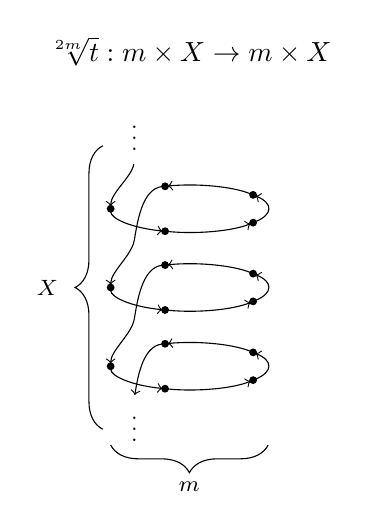
\begin{tikzpicture}
    \node (A) at (0,4) {$\sqrt[\uproot{2}m]t:{\bn m\times X}\to{\bn m\times X}$};
    \foreach \y in {0,1,2}
    { \begin{scope}[shift={(0,\y)}]
        \foreach \x in {0,...,4}
        { \node[fill,circle,inner sep=1pt] at (180+72*\x:1 and .3) {}; }
        \foreach \x in {0,...,3}
        { \draw[->,shorten <=1pt,shorten >=1pt]
          (180+72*\x:1 and .3) arc(180+72*\x:252+72*\x:1 and .3); }
      \end{scope} }
    \foreach \y in {1,2}
    { \begin{scope}[shift={(0,\y)}]
        \draw[->,shorten <=1pt,shorten >=1pt] (108:1 and .3)
        .. controls ++( 5:-.3) and ++(80:.2) .. (-.7,-.4)
        .. controls ++(80:-.2) and ++(90:.2) .. (-1,-1);
      \end{scope} }
    \draw[->,shorten <=1pt,shorten >=1pt] (108:1 and .3)
    .. controls ++( 5:-.3) and ++(80:.2) .. (-.7,-.4);
    \node (dz) at (-.7,-.7) {\footnotesize$\vdots$};
    \begin{scope}[shift={(0,3)}]
      \draw[->,shorten <=1pt,shorten >=1pt] (-.7,-.4)
      .. controls ++(80:-.2) and ++(90:.2) .. (-1,-1);
      \node (da) at (-.7,0) {\footnotesize$\vdots$};
    \end{scope}
    \draw [decorate,decoration={brace,amplitude=10pt}]
    (-1.1,-.8) -- (-1.1,2.8) node [black,midway,xshift=-20pt] {\footnotesize $X$};
    \draw [decorate,decoration={brace,amplitude=10pt}]
    (1,-1) -- (-1,-1) node [black,midway,yshift=-15pt] {\footnotesize $\bn{m}$};
  \end{tikzpicture}
  \caption{The $m$\th root $\sqrt[\uproot{2}m]t$
    of a function $t: X\to X$,
    here illustrated in the case $m=5$.}\label{fig:root}
\end{marginfigure}

\begin{construction}\label{con:root}
  For any type $X$ and $t:X\to X$, we define the $m$\th \emph{root}
  \[
    {\textstyle\sqrt[\uproot{2}m]t} : {\bn m\times X} \to {\bn m\times X}.
  \]
\end{construction}
\begin{implementation}{con:root}
  We set
  \[
    {\textstyle\sqrt[\uproot{2}m]t}(k,x)\defeq
    \begin{cases}
      (k+1,x)& \text{for $k<m-1$ and}\\
      (0,t(x))& \text{for $k=m-1$}.
    \end{cases}
  \]
\par \vspace{-1.5\baselineskip}
\qedhere
\end{implementation}
Only one $m$\th of the time does $\sqrt[\uproot{2}m]t$ use $t:X\to X$,
the rest of the time it applies the successor in $\bn m$.
Indeed, iterating $\sqrt[\uproot{2}m]t$
we get $(\sqrt[\uproot{2}m]t)^m(k,x)=(k,t(x))$;
hence the term ``$m$\th root'' is apt.

\begin{definition}
  The \emph{formal $m$\th root function} is defined by:
  \[
    \cdg{m}:\sum_{X:\UU}(X\to X)\to\sum_{X:\UU}(X\to X),\qquad
    \cdg{m}(X,t)\defeq(\bn m\times X,{\textstyle\sqrt[\uproot{2}m]t}).\qedhere
  \]
\end{definition}
\noindent We use $\rho$ for ``root'' to denote this incarnation
of the degree $m$ function.

\begin{lemma}\label{lem:root-pres-equiv}
  If $t:X\to X$ is an equivalence,
  then so is $\sqrt[\uproot{2}m]t : \bn m\times X \to \bn m\times X$.
\end{lemma}
\begin{proof}
  On one hand, an element in  $(\sqrt[\uproot{2}m]t)(\ell,y) = (0,x)$ consists
  of the assertion that  $\ell=m-1$ and an element in $t(y)=x$,
  so  $(\sqrt[\uproot{2}m]t)^{-1}(0,x)$ is equivalent
  to $t^{-1}(x)$, which is contractible if $t$ is an equivalence.

  On the other, if $k:\bn m$ is not $0$,
  then an element in $(\sqrt[\uproot{2}m]t)(\ell,y)=(k,x)$
  consists of the assertion that $\ell+1=k$ and an element in $y=x$,
  and so $(\sqrt[\uproot{2}m]t)^{-1}(k,x)$ is equivalent
  to the contractible type $\sum_{y:X}y=x$.\marginnote{%
    Of course, it's also quite easy to write down an inverse
    of $\sqrt[\uproot{2}m]{t}$ given an inverse of $t$.}
\end{proof}

\begin{lemma}
  If $(X,t)$ is a cycle, then so is $\cdg{m}(X,t)$.
\end{lemma}
\begin{proof}
  Clearly, $\bn m\times X$ is \nonempty if $X$ is.
  And we already know $\sqrt[\uproot{2}m]{t}$ is an equivalence if $t$ is.

  Suppose $(k,x),(k',x'):\bn m\times X$.
  We need to show the proposition that there merely exists $n:\zet$
  with $(k',x') = \bigl(\sqrt[\uproot{2}m]t\bigr)^n(k,x)$.
  Let $n:\zet$ be such that $x' = t^n(x)$.
  Then $(\sqrt[\uproot{2}m]t)^{nm}(k,x) = (k,t^n(x)) = (k,x')$,
  so if $k=k'$ we're done.
  Assume $k<k'$. Then $(\sqrt[\uproot{2}m]t)^{k'-k}(k,x') = (k',x')$,
  so $(\sqrt[\uproot{2}m]t)^{nm+k'-k}(k,x) = (k',x')$, as desired.
  The case $k>k'$ is similar.
\end{proof}

The question now arises: how does $\cdg{m}$ act on the components of $\Cyc$,
and what can we say about the preimages $\cdg{m}^{-1}(X,t)$
for an arbitrary cycle $(X,t)$?

The first part is easy, since the product of $\bn m$ with an $n$-element set
is an $mn$-element set. We set $\pt_n \defeq (\bn n,\zs) : \Cyc_n$.
\begin{lemma}
  The degree $m$ function restricts to give pointed maps
  \[
    \cdg{m} : \Cyc_n \ptdto \Cyc_{mn} \quad\text{and}\quad
    \cdg{m} : \Cyc_0 \ptdto \Cyc_0.
  \]
\end{lemma}
\begin{proof}
  Note\marginnote{%
    In terms of iterated addition, we have
    $\varphi(k,r) = (z \mapsto z+m)^r(k)$.}
  that the function $\varphi : (\bn m\times \zet) \to \zet$
  given by $\varphi(k,r)=k+mr$ is an equivalence,
  with inverse given by Euclidean division by $m$.
  Moreover, we have ${\varphi\!\sqrt[\uproot{2}m]\zs} = {\zs\varphi}$, since
  \[
    \varphi\bigl(\!\sqrt[\uproot{2}m]\zs(k,r)\bigr)
    = k+1+mr = \zs(\varphi(k,r))
    \quad\text{for all $(k,r):\bn m\times \zet$}.
  \]
  This shows that $\varphi$ gives an identification of infinite cycles
  $(\bn m\times\zet, \sqrt[\uproot{2}m]\zs) = (\zet,\zs)$,
  and hence the $m$\th root construction maps the component $\Cyc_0$ to itself.

  Taking remainders modulo $mn$, we see that $\varphi$ restricts
  to give an equivalence $\bn m \times \bn n \we \sum_{k:\zet}(k<mn)$,
  and hence an identification of cycles $\cdg{m}(\pt_n) = \pt_{mn}$,
  showing that $\cdg{m}$ maps the component $\Cyc_n$ to the component $\Cyc_{mn}$.
\end{proof}

We now analyze how $\cdg{m}$ acts on paths.
Let $\pathpair{\etop{e}}{!}:(X,t)=(X',t')$.
Since $\cdg{m}$ maps first components $X$ to $\bn m\times X$, we get that
the first projection of $\ap{\cdg{m}}\pathpair{\etop{e}}{!}$ is
$\overetop{\id\times e} : (\bn m\times X) = (\bn m\times X')$.
We are particularly interested in the case of the loops,
that is, $\pathpair{\etop{e}}{!}:(X,t)=(X,t)$.
We calculate $(\id\times e)(k,x) = (k,e(x))$,
which by the property of the $m$\th root is equal to $(\sqrt[\uproot{2}m]e)^m(k,x)$.
In particular, if we take $e\defeq t^{-1}$,
then we get $(\id\times t^{-1}) = (\sqrt[\uproot{2}m]{t^{-1}})^m$, which means that
$\ap{\cdg{m}}\pathpair{\etop{t}^{-1}}{!}$ is indeed the $m$\th power of the
generating loop at the image cycle $\cdg{m}(X,t)$.
In particular, this holds for the standard infinite cycle $(\zet,\zs):\Cyc_0$
and the standard $n$-cycle $(\bn n,\zs):\Cyc_n$.

Why does $\cdg{m}:\Cyc_0\to\Cyc_0$
correspond to the $m$-fold \covering we defined in \cref{def:mfoldS1cover}?
This is encapsuled by the fact that under the equivalence $c:\Sc\to C$, the two $m$-fold covers agree in the sense that the two functions given as composites in
\[
  \begin{tikzcd}
    \Sc\ar[r,"c"]\ar[d,"\dg{m}"'] & \Cyc_0\ar[d,"\cdg{m}"] \\
    \Sc\ar[r,"c"] & \Cyc_0
  \end{tikzcd}
\]
are equal; we need an element in
\[
  \cdg{m}c=_{\Sc\to\Cyc_0}c\,\dg{m}.
\]
Under the equivalence
\[
  \ev_{\Cyc_0}:(\Sc\to\Cyc_0)\we \sum_{(X,t):\Cyc_0}\bigl((X,t)=(X,t)\bigr)
\]
of \cref{lem:freeloopspace},
the composite $c\,\dg{m}$ is given by $\bigl((\zet,\zs),\zs^{-m}\bigr)$
and the composite $\cdg{m}c$ is given by
$\bigl((\bn m\times\zet,\sqrt[\uproot{2}m]{\zs^{-1}}),\id\times\zs^{-1}\bigr)$:
we must produce an element in
\[
  \Bigl((\bn m\times\zet,\sqrt[\uproot{2}m]{\zs^{-1}}),\id\times\zs^{-1}\Bigr)
  = \bigl((\zet,\zs),\zs^{-m}\bigr).
\]
Consider the equivalence  $\varphi: (\bn m\times \zet)\to\zet$ with $\varphi(k,n)=k+mn$ discussed above.
Since transport of $\sqrt[\uproot{2}m]\zs$ along $\varphi$ is exactly $\zs$ (\ie $\varphi\!\sqrt[\uproot{2}m]\zs=\zs\varphi$;
note the way we formulate this so that we don't need to talk about the inverse of $\varphi$\footnote{%
  Of course, the inverse of $\varphi$ maps $z:\zet$ to the remainder and the integer quotient of $z$ under Euclidean division by $m$, cf.~\cref{lem:euclid-div}.})
we get an identification that we also call
$\varphi: \bigl(\bn m\times\zet,\sqrt[\uproot{2}m]{\zs^{-1}}\bigr)=(\zet,\zs^{-1})$.  Likewise, transport of $\id\times\zs$ along $\varphi$ is $\zs^m$,
so that $\varphi$ lifts to an element in
$\bigl((\bn m\times\zet,\sqrt[\uproot{2}m]{\zs^{-1}}), \id\times\zs^{-1}\bigr)
= \bigl((\zet,\zs),\zs^{-m}\bigr)$.

\begin{xca}\label{xca:pointed-maps-circle}
Verify $\cdg{m}c=_{\Sc\ptdto\Cyc_0}c\,\dg{m}$ in case all maps are taken to be pointed.
\end{xca}

So we know that the fiber of $\cdg{m}$ at an infinite cycle $(X,t)$
is an $m$-element set. In fact, we can identify this set as
$X/m \defeq X/\sim_m$ where $\sim_m$ is the equivalence relation that
identifies points that are a distance $mr$ apart, for some $r:\zet$.
Formally, let $x\sim_m x'$ if and only if $\exists_{r:\zet}(x'=t^{mr}(x))$.
(Such an $r$ is unique if it exists.)
Indeed, the fiber is
\[
  \sum_{(Y,u):\Cyc_0}\bigl((X,t) = (\bn m\times Y, \sqrt[\uproot{2}m]{u})\bigr).
\]
The equivalence is obtained by sending an equivalence class $Y$ to
the corresponding infinite cycle $(Y,u^m)$ together with the
natural identification $(X,t) = (\bn m\times Y, \sqrt[\uproot{2}m]{u^m})$.
See \cref{thm:fiber-cdg} below for a careful proof of a more general statement.

The reader will no doubt have noticed that $X/m$ is a \emph{finite cycle}.
We'll return to the significance of this below.

Our next step is to identify the fiber of $\cdg{m}$ over a general cycle $(X,t)$.
Classically, the remaining cases are those of finite $n$-cycles,
but it's illuminating to be a bit more general.
Note that the equivalence relation $\sim_m$ defined above for an infinite cycle
makes sense for all cycles.

\begin{lemma}\label{lem:sum-cycle-point-contr}
  For any order $d:\Order$, the type $\sum_{(X,t):\Cyc_d}X$ is contractible,
  where $\Cyc_d$ denotes the component of $\Cyc$ consisting
  of cycles of order $d$.
\end{lemma}
\begin{proof}
  This is relatively straight-forward from \cref{lem:IdCycle}.
  The type in question is nonempty since all cycles have a nonempty underlying set,
  so it suffices to prove the type is a proposition.
  So let $(X,t),(X',t')$ be cycles of order $o$, and take $x:X$ and $x':X$.
  An identification $((X,t),x) = ((X',t'),x')$ is given by an equivalence of
  cycles $e : (X,t)=(X',t')$ with $e(x)=x'$.
  But evaluation at $x$ induces an equivalence
  $\bigl((X,t)=(X',t')\bigr) \simeq X'$,
  so there exists a unique $e$ with $e(x)=x'$.
\end{proof}
\begin{lemma}\label{lem:m-root-id}
  For any cycle $(X,t)$, if $(\sqrt[\uproot{2}m]{t})^n = \id$,
  then $m$ divides $n$, \ie $n=mq$ for some $q:\zet$, and $t^q=\id$.
  In other words, $m$ divides the order of $\sqrt[\uproot{2}m]{t}$.
\end{lemma}
This follows simply by looking at the first component,
where $\sqrt[\uproot{2}m]{t}$ acts as the successor operation on $\bn m$.

We're almost ready to identify the fiber of $\cdg{m}$ at a cycle $(X,t)$.
We know that the fiber is \nonempty only if $m$ divides the order.
A key ingredient for the converse is the following.
\begin{lemma}\label{lem:X-mod-m-chosen}
  Let $(X,t):\Cyc$ be a cycle with a chosen point $x_0:X$
  and with order divisible by $m$.
  Then the map $f : \bn m \to X/m$, $f(k) \defeq [t^k(x_0)]$
  is an equivalence.
\end{lemma}
\begin{proof}
  Fix an equivalence class $V:X/m$ and consider its preimage under $f$,
  $f^{-1}(V) \jdeq \sum_{k:\bn m}(V=[t^k(x_0)])$.
  The contractibility of this type is a proposition, so we may choose
  $x:X$ with $V=[x]$.
  Then $(V=[t^k(x_0)])\equiv([x]=[t^k(x_0)])\equiv(x\sim_m t^k(x_0))$.
  So we need to show that $\sum_{k:\bn m}(x\sim_m t^k(x_0))$ is contractible.
  More simply, we need to show that there is a unique $k$ with $x\sim_m t^k(x_0)$.
  Since $(X,t)$ is a cycle, we may further choose $n:\zet$ with $x=t^n(x_0)$.
  By Euclidean division, write $n=qm+r$ with $q:\zet$, $r:\bn m$.
  Then $x = t^n(x_0) \sim_m t^r(x_0)$, so we have our center.
  Let $k:\bn m$ also satisfy $x\sim_m t^k(x_0)$.
  We need to show the proposition $k=r$.
  But $t^{r-k}(x_0) \sim_m x_0$, so we may take $q:\zet$ with $t^{qm+r-k}(x_0)=x_0$.
  Since $m$ divides the order of $t$, this implies $r=k$, as desired.
\end{proof}
Now we have all the pieces needed to prove the main result.
\begin{theorem}\label{thm:fiber-cdg}
  For \emph{any} cycle $(X,t)$, the preimage $\cdg{m}^{-1}(X,t)$
  is equivalent to $P\times X/m$,
  where $P\defeq (m \mid \ord(t)) \jdeq (H_t \subseteq m\zet)$
  expresses that $m$ divides the order of $t$.
\end{theorem}
\begin{proof}
  We'll use \cref{lem:weq-iso}, and we first define the function
  \[
    g : \cdg{m}^{-1}(X,t) \to P\times X/m,
  \]
  by mapping $(Y,u)$ and an identification of cycles
  $e : (X,t) = (\bn m\times Y,\sqrt[\uproot{2}m]{u})$
  to the proof of $P$ from \cref{lem:m-root-id}
  and the class $V_e\defeq [e^{-1}(0,y)]:X/m$, for any $y:Y$.
  Note that this doesn't depend on $y$, and as a subset of $X$,
  $V_e=\setof{x:X}{\fst(e(x))=0}$.

  In the other direction, to define the function
  \[
    h : P\times X/m \to \cdg{m}^{-1}(X,t),
  \]
  fix an equivalence class $V:X/m$,
  and assume that $m$ divides the order of $t$.
  Then we have, with a bit of abuse of notation, the cycle $(V,t^m)$,
  where we also write $V$ for the type of elements in $X$ that lie in the class $V$,
  and $t^m$ is the restriction of this power of $t$ to $V$.\footnote{%
    If $x$ lies in $V$, then so does $t^m(x)$.}
  We also need an identification
  $(X,t)=(\bn m\times V,\sqrt[\uproot{2}m]{t^m})$.
  This we define via a map $e : \bn m\times V \to X$, $e(k,x) \defeq t^k(x)$.
  This is an equivalence as long as the orders match.
  So let $n:\zet$, and assume first that $t^n=\id$.
  Then $P$ implies that we may write $n=qm$ for some $q:\zet$,
  so
  \[
    (\sqrt[\uproot{2}m]{t^m})^n
    = (\sqrt[\uproot{2}m]{t^m})^{qm}
    = (\id \times t^m)^q = (\id \times t^{qm}) = \id.
  \]
  Conversely, we know from \cref{lem:m-root-id} again,
  that if $(\sqrt[\uproot{2}m]{t^m})^n=\id$,
  then we may write $n=qm$ for some $q:\zet$,
  and $(t^m)^q=\id$, which by \cref{lem:cycle-order-point-ap}
  implies that $t^n = \id$.

  Straight from these definitions, we see that $g\circ h=\id$.
  We leave to the reader to check that $h\circ g=\id$.
\end{proof}

\section{Getting our cycles in order}
\label{sec:cycles-order}

{\color{casblue} TODO: Exposition and figures

\begin{xca}
  Prove that if $(X,t),(Y,u)$ are cycles, $x_0:X$,
  then the type of maps $f : (X,t) \to (Y,u)$ is equivalent to $P\times Y$,
  where $P\defeq(\ord(u) \mid \ord(t)) \jdeq (H_t \subseteq H_u)$.
\end{xca}

Thus, an order $p$ divides an order $q$ if and only if
there is a map of cycles from a cycle of order $q$
to a cycle of order $p$.
\begin{theorem}
  The partially ordered set $(\Order,|)$ is a lattice
  with least element the finite order $1$
  and greatest element the infinite order, represented by the number $0$,
  and meets and joins given by “gcd” and “lcm”, respectively.
\end{theorem}

subgroups of $\constant{C}_n = \constant{C}_k$ where $k | n$
connected set bundles of $\Cyc_n$

\subsection{More TODO}

\begin{itemize}
\item Classify connected \coverings over $\Cyc_n$.
\item Universal property of $\Cyc_n$ among groupoids.
\item Bijective proof of $mn = \lcm(m,n)\times\gcd(m,n)$ via the product of cycles.
  Chinese remainder stuff.
\item Somehow sneak in totatives and automorphisms of cyclic groups?
\end{itemize}
}

\subsection{Universal property of $\Cyc_n$}

This section is devoted to showing that maps out of $\Cyc_n$ into a groupoid
are equivalently given by the choice of a point togetehr with a symmetry of
order $n$: that is any map $\Cyc_n \to A$ is fully determined by a point $a$ of
the groupoid $A$ together with a symmetry $\sigma:a=a$ such that
$\sigma^n=\refl a$.

Recall that $\Cyc_n$ contains the point $\pt_n \defequi (\bn n, \zs)$. This
point has a symmetry $\sigma_n \defequi (\zs, !)$ whose second projection is a
proof that $\zs\zs = \zs\zs$ \marginnote{Should we take $(\inv \zs,!)$ instead to
match the choice in the case $\Cyc_0$?}. 
%
Recall also from \cref{cor:id-m-cycle} that all elements of $\pt_n = \pt_n$ are
of the form $\sigma_n^i$ for $i=0,\dots,n-1$.

Given a groupoid $A$, and a map $f :
\Cyc_n \to A$, one can consider $f(\pt_n)$ and $\ap f (\sigma_n): f(\pt_n) =
f(\pt_n)$. Transporting a proof of the equation $\refl {\pt_n} = \sigma_n^n$ in
$\Cyc_n$ through $f$, one gets a proof of $\refl {f(\pt_n)} =
\ap f(\sigma_n)^n$. Hence, the following map is well-defined:
\begin{displaymath}
  \ev_{n,A} : (\Cyc_n \to A) \to \sum_{a:A}\sum_{\sigma:a=a}\refl a = \sigma^n,\quad
  f \mapsto (f(\pt_n), \ap f (\sigma_n), !)
\end{displaymath}

\begin{theorem}
  For any groupoid $A$, the map $\ev_{n,A}$ is an equivalence.
  \label{prop:ump-cycn-into-groupoids}
\end{theorem}
\begin{proof}
  Let $a:A$ and $\sigma:a=a$ such that $\refl a = \sigma^n$ holds.
  One wants to prove that the fiber 
  \begin{displaymath}
    \sum_{f:\Cyc_n \to A} (a,\sigma, !) = \ev_{n,A}(f)
  \end{displaymath}
  is contractible. Hence we first need to craft a function $f:\Cyc_n \to A$
  such that there is $p:a=f(\pt_n)$ such that $\ap f (\sigma_n) \cdot p = p
  \cdot \sigma$.

  In order to do so, we will craft a function $f:\Cyc_n \to A$ together with a
  function $\hat p_x: \pt_n = x \to a = f(x)$ for each $x:\Cyc_n$ such that
  $\hat p_x(\blank\sigma_n) = \hat p_x(\blank) \sigma$. By setting $p \jdeq \hat
  p_{\pt_n}(\refl {\pt_n})$, we would have succeeded. Indeed, path induction on
  $\alpha: x = x'$ shows that $\hat p_{x'}(\alpha \blank) = \ap f (\alpha) \hat
  p_x(\blank)$ on one hand, and the hyptohesis on $\hat p$ proves that $\hat
  p_{\pt_n} (\blank) \sigma = \hat p_{\pt_n}(\blank \sigma_n)$ on the other
  hand. This leads to the chain of equations:
  \begin{displaymath}
    p \sigma = \hat p_{\pt_n}(\refl {\pt_n}) \sigma = \hat p_{\pt_n}(\refl {\pt_n}\sigma_n) = \hat p_{\pt_n}(\sigma_n\refl {\pt_n}) = \ap f (\sigma_n) \hat p_{\pt_n}(\refl {\pt_n}) = \ap f (\sigma_n) p 
  \end{displaymath}

  It remains to craft the promised $f$ and $\hat p$. For each $x:\Cyc_n$, consider the type
  \begin{displaymath}
    T(x) \defequi \sum_{b:A}\sum_{\pi: \pt_n = x \to a = b} \pi(\blank\sigma_n) = \pi(\blank) \sigma
  \end{displaymath}
  One claims that $T(x)$ is contractible. To prove this proposition for $x$
  ranging over the connected type $\Cyc_n$, it is enough to only prove it for
  $x \jdeq \pt_n$. However, as every element of $\pt_n = \pt_n$ can be written
  as $\sigma_n^i$ for some $i:\bn n$, one gets:
  \begin{displaymath}
    T(\pt_n) \weq \sum_{b:A}\sum_{\pi: \bn n \to a = b} \pi(\blank) = \pi(0)\sigma^{\blank} \weq \sum_{b:A} a = b \weq 1
  \end{displaymath}
  One gets $f(x)$ by selecting a center of contraction for each $x:\Cyc_n$ and the function $\hat p_x$ is then defined as the first projection of the second component of this center of contraction. 
\end{proof}

\section{Old material yet to be integrated}
\label{sec:deckS1}

There are many other instances of the $m$\th root construction, \cref{con:root},
which is of independent interest.
We record the following for future reference.
\begin{definition} \label{def:Zetmodm}
Let $m$ be a positive integer.
The element $\zet/m:\sum_{X:\Set}(X=X)$ has first projection $\bn m\times\bn 1$ and
second projection $\sqrt[\uproot{2}m]{\refl{\bn 1}}$.
\end{definition}
\noindent
This realizes the cycle $0\mapsto1\mapsto\dots\mapsto m-1\mapsto 0$ in $\bn m$,
and so models ``modular arithmetic''.

% In this section we prove the following result.
The term ``cyclic'' in the chapter heading refers to the fact that we show
that the symmetries of \coverings are determined by iterations of a single symmetry.

\begin{remark}
Since we are interested in the symmetries of particular \coverings it is
good to spell out some details.
By \cref{lem:isEq-pair=} the identity type $(A,f,!)=(A',f',!)$ of
two \coverings over the type $B$ is equivalent to
\[
\sum_{p_A:A=_{\UU}A'}(\pathover{f}{X\mapsto(X\to B)}{p_A}{f'}).
\]
The latter type is by \cref{def:pathover-trp} and \cref{lem:trp-in-function-type}
with $X\jdeq\UU,~Y\jdeq\id_{\UU}$ and $Z$ constant $B$, and the remark
after \cref{def:idtoeq} that $\ptoe{p}_A = \trp[\id_{\UU}]{p_A}$, equivalent to
\[
\sum_{p_A:A=_{\UU}A'}(f =_{A\to B}f'\ptoe{p}_A).
\]
The situation can be depicted as
\[
  \begin{tikzcd}[baseline=(O.base)]
    A\ar[rr,eqr,"p_A"]\ar[dr,"f"'] & & A'\ar[dl,"f'"] \\
    & |[alias=O]| B. &
  \end{tikzcd}\qedhere
\]
\end{remark}

% We start by investigating the symmetries of the universal \covering of the circle,
% since this case is simpler than that of the $m$-fold \coverings.
% Some easy observations will pave the way.

% First, for any types $X,Y$
% define $C_{Y,X} : X\to (Y\to X)$ to map any $x:X$ to the map $Y\to X$
% that is constant $x$, that is, $C_{Y,X}(x)\defeq c_x$.
% %We may leave out the subscripts of the map $C$. (confusion with type C)
% Clearly, $C_{\bn{1},X}$ is an equivalence from $X$ to $\bn{1}\to X$,
% which induces an equivalence from $x=x$ to $C_{Y,X}(x) = C_{Y,X}(x)$
% for any $x:X$.

% Second, we have by UA that $\bn{1}=\bn{1}$ is contractible
% and mapping $e: f=g$ to $(\refl{\bn{1}},e)$ is a equivalence from
% $f=g$ to $\sum_{i:\bn{1}=\bn{1}} (\pathover{f}{\_\mapsto X}{i}{g})$
% for all $f,g:\bn{1}\to X$.

% Third, we have the equivalence from \cref{lem:isEq-pair=}.
% Combining these three equivalences in the special case of the point $\base:\Sc$ we get:
% \[
% (\base=\base) \equiv (c_\base=c_\base) \equiv
% \sum_{i:\bn{1}=\bn{1}} (\pathover{c_\base}{\_\mapsto \Sc}{i}{c_\base}) \equiv
% ((\bn{1},c_\base)=_{\hat\Sc}(\bn{1},c_\base)).
% \]
% The trace is $p \mapsto \ap{C_{\bn{1},X}}(p) \mapsto
% (\refl{\bn{1}},\ap{C_{\bn{1},X}}(p)) \mapsto \pathpair{\refl{\bn{1}}}{\ap{C_{\bn{1},X}}(p)}$.
% Applying this trace with $p\defeq\Sloop$ we obtain an additive unit for
% all these types that are equivalent to $\zet$.
Recall that for any type $X$ and element $x:X$, $\cst x$ denotes the
function $\bn 1\to X$ defined by $\cst x (\ast) \defequi x$ on the
unique element $\ast: \bn 1$. In particular,
$\cst \base : \bn 1 \to \Sc$ denotes the universal \covering of $\Sc$.

\begin{theorem}~%
  \label{thm:coveringsofS1}
  \begin{enumerate}
  \item \label{item:univ-cover-Sc-Z}%
    There is an equivalence
    $\Sc \weq \conncomp {\SetBundle(\Sc)} {\cst \base}$ mapping
    $\base$ to $(\cst \base, \trunc{\refl {\cst \base}})$.

    In particular, there is a symmetry
    \[
      Q^1:\cst\base=_{\SetBundle(\Sc)}\cst\base
    \]
    such that every symmetry of $\cst\base$
    (as a \covering over $\Sc$)
    can be identified with $(Q^1)^k$ for a unique $k:\zet$.

  \item \label{item:setbundle-mcover}%
    For a positive integer $m$, the set
    $\dg{m}=\dg{m}$ of symmetries of the
    $m$-fold \covering of the circle is equivalent to the finite type
    $\bn m$.

    Furthermore, there is a symmetry
    \begin{displaymath}
      Q^1:\dg{m}=_{\SetBundle(\Sc)}\dg{m}
    \end{displaymath}
    so that every symmetry of $\dg{m}$ (as set bundle over
    $\Sc$) can be identified with $(Q^1)^i$ for a uniquely determined $k$ between
    $0$ and $m-1$. In other words, following \cref{def:Zetmodm},
    \begin{displaymath}
      \conncomp{\SetBundle(\Sc)}{\dg{m}} \weq \conncomp{\left(\sum_{X:\Set}X=X\right)}{\zet/m}.
    \end{displaymath}

  \end{enumerate}
 \end{theorem}
\begin{remark}\label{rem:thenonuniquenessofgeneratorsofmodulararithmetic1}
  The symmetries called $Q^1$ in \cref{thm:coveringsofS1} are not
  uniquely determined by the stated property.  In the case of the
  universal \covering there are two candidates and for the $m$-fold
  \covering there are as many as there are positive integers less than
  $m$ that does not divide $m$.  This behavior has number theoretic
  consequences and origins and will be investigated further when we
  have the proper machinery to put it to good use.
\end{remark}

\begin{proof}
  Let us first prove \ref{item:univ-cover-Sc-Z}. Through
  \cref{lem:S1-delooping}, it is enough to find an equivalence
  $(\base = \base) \weq (\cst\base =_{\SetBundle(\Sc)} \cst\base)$
  which preserves reflexivity and composition of paths. It is obtained
  as the composition
  \begin{displaymath}
    \left(\base =_{\Sc} \base\right) \weq \left( \cst\base=_{\bn 1\to \Sc}\cst\base \right)
    \weq \left( \cst\base =_{\SetBundle(\Sc)} \cst\base \right)
  \end{displaymath}
  where the first equivalence is given by induction on $\bn 1$ and
  function extensionality, and the second one is mapping a path $e$ to
  the path $(\refl{\bn 1}, e)$. Both equivalences clearly preserve
  reflexivity paths and composition of paths, hence so does their
  composition.

  Let us move on to \ref{item:setbundle-mcover}. %
  First, let us emphasize that we are interested in the symmetries of
  $\dg{m}$ \emph{as a set bundle}, meaning we shall explore
  the loops $(\Sc,\dg{m}) =_X (\Sc,\dg{m})$ in the type
  $\SetBundle(\Sc)$.
  Because $\SetBundle(\Sc)$ is a subtype of $\sum_{A:\UU}A\to \Sc$, it
  is enough to determine the symmetries of $(\Sc,\dg{m})$ in this later
  type (cf.\ \cref{lem:subtype-eq-=}). This is unfolded as:
  \begin{displaymath}
    D_m \defequi \sum_{g:\Sc = \Sc}\dg{m} =_{\Sc \to \Sc} \dg{m}\ptoe g
  \end{displaymath}
  Recall the equivalence $c: \Sc \to C$ of
  \cref{thm:S1bysymmetries}. Then the transport along $\etop c$ in the
  type family $X\mapsto (\Sc=X)$ is an equivalence from $(\Sc = \Sc)$
  to $(\Sc = C)$. Composing with univalence, we get that an
  equivalence $(\Sc=\Sc) \to (\Sc \weq C)$ mapping
  $g\mapsto c\ptoe{g}$, with inverse
  $t \mapsto \overetop{\inv{c} t}$.
  Hence, by following \cref{xca:sum-equiv-base} we get
  \begin{displaymath}
    D_m \weq  \sum_{t:\Sc \weq C} \dg{m} =_{\Sc\to \Sc} \dg{m}\inv c t.
  \end{displaymath}
  Then, denoting $\cdg{m}: C \to C$ for the $m$-fold cover of $C$,
  \begin{displaymath}
    \begin{split}
      (\dg{m} =_{\Sc\to \Sc} \dg{m}\inv c t) %
      &\weq (c \dg{m} =_{\Sc\to C} c \dg{m} \inv c t)
      \\
      &\weq (\cdg{m}c =_{\Sc\to C} \cdg{m} t)
    \end{split}
  \end{displaymath}
  where the first equivalence holds because $c$ is an equivalence, and
  the second because $\cdg{m}c =_{\Sc\to C} c \dg{m}$ has been
  proved in \cref{exa:mfoldCcover}.
  Then if we write
  \begin{displaymath}
    F_m \defequi \sum_{t:\Sc \weq C}(\cdg{m}c =_{\Sc\to C} \cdg{m} t),
  \end{displaymath}
  one gets that $D_m \weq F_m$ and we can now concentrate on proving that
  $F_m \weq \bn m$.

  Let us first sketch the proof in three steps:
  \begin{enumerate}[label={\sc Step \arabic*}.]
  \item We shall describe the elements of $F_m$ as basically tuples
    $(Y,g,q)$ with $(Y,g)$ in the subtype $C$ of $\sum_{X:\UU}(X=X)$
    and $q:\bn m\times \zet = \bn m\times Y$ such that $q$ satisfies
    certain propositional equations, denoted $E(q)$ here.
  \item We shall then give a characterization of these elements
    $(Y,g,q)$ in the case where $Y$ is $\zet$ and $g$ is $\etop
    s$. This characterization will give $q$ (viewed as an equivalence)
    the following form:
    \begin{displaymath}
      q_{i,n}: (j,z) \mapsto {\sqrt[\uproot{2}m]s}^j(i,n+z)
    \end{displaymath}
    In particular, it can be seen that
    $(\zet,\etop s,q_{i,n}) = (\zet,\etop s,q_{i,0})$ in $F_m$.
  \item Finally we shall define a map $\psi: \bn m \to F_m$ properly
    as $i\mapsto (\zet,\etop s,q_{i,0})$ and prove that it is an
    equivalence. It means that given $(Y,g,!):C$, one has to show
    \begin{displaymath}
      P(Y,g) \defequi \prod_{q:\bn m \times \zet = \bn m \times Y}E(q)\to\iscontr(\inv{\psi}(Y,g,q))
    \end{displaymath}
    where $E(q)$ is as in step 1. The dependent product is valued in
    propositions so $P(Y,g)$ itself is a proposition. By definition of
    $C$, $(Y,g)$ lies in the same connected component as $(Z,\etop s)$
    in $\sum_{X:\UU}X=X$, so using \cref{xca:component-connected},
    $P(Y,g)$ holds as soon as $P(Z,\etop s)$ holds. Otherwise put, it
    is enough to prove the contractibility of the fiber of $\psi$ at
    elements of $F_m$ of the form $(Z,\etop s,q)$ for which step 2
    shows that $q$ must be one of the $q_{i,n}$ for some $(i,n)$. This
    $i$, together with the essentially unique proof that
    $(\zet,\etop s, q_{i,n}) = (\zet,\etop s, q_{i,0})$, is then
    easily seen to be a center of contraction for the fiber
    $\inv\psi(Z,\etop s, q)$.
  \end{enumerate}

  {\sc Step 1.} An element of $F_m$ is given by a map $t:\Sc \to C$
  together with a term $!:\isEq(t)$ and a proof
  $Q: \cdg{m}c = \cdg{m}t$. Now such a $t$ can be reduced through
  the universal property of $\Sc$ to the data of
  $t(\base)\defequi (Y,g,!)$ and
  $t(\Sloop)\defis (p,!,!): (Y,g,!) =_C (Y,g,!)$. Under identification
  through the universal property of $\Sc$, $\cdg{m}c$ is given by
  \begin{displaymath}
    \begin{split}
      &\cdg{m}c(\base) \defequi (\bn m\times \zet,\sqrt[\uproot{2}m] {\etop s},!)\\
      &\cdg{m}c(\Sloop) \defis (\id \times {\etop s},!,!): (\bn
      m\times \zet,\sqrt[\uproot{2}m] {\etop s},!) =_C (\bn m\times
      \zet,\sqrt[\uproot{2}m] {\etop s},!)
    \end{split}
  \end{displaymath}
  and similarly $\cdg{m}t$ is given by
  \begin{displaymath}
    \begin{split}
      &\cdg{m}t(\base) \defequi (\bn m\times Y,\sqrt[\uproot{2}m] g,!)\\
      &\cdg{m}t(\Sloop) \defis (\id \times p,!,!): (\bn m\times
      Y,\sqrt[\uproot{2}m] g,!) =_C (\bn m\times Y,\sqrt[\uproot{2}m] g,!)
    \end{split}
  \end{displaymath}
  By function extensionality and $\Sc$-induction, $Q$ becomes then a
  term $q:\bn m\times \zet = \bn m\times Y$ such that the two
  following propositions hold, whose product is denoted $E(q)$:
  \begin{displaymath}
    {\sqrt[\uproot{2}m]g} \circ q = q \circ \sqrt[\uproot{2}m]{\etop s}%
    \quad\text{and}\quad%
    q \circ (\id \times {\etop s}) = (\id \times p) \circ q.%
  \end{displaymath}
  Remark that repeated applications of the first equation imply that
  such a $q$ is completely determined by
  $\ptoe q (0,0): \bn m\times Y$: indeed for all $j\in\bn m$ and
  $z\in\zet$
  \begin{displaymath}
    \ptoe q (j,z) = \ptoe q ( \sqrt[\uproot{2}m]s^{j+zm} (0,0))%
    = \sqrt[\uproot{2}m]g^{j+zm} \ptoe q(0,0)%
  \end{displaymath}
  Remark also for future references that the proposition $p=g$ holds:
  indeed,
  \begin{displaymath}
    \id \times p = q \circ (\id \times {\etop s}) \circ q^{-1}
    = (q\sqrt[\uproot{2}m]{\etop s}q^{-1})^m = (\sqrt[\uproot{2}m]g)^m = \id \times g.
  \end{displaymath}

  {\sc Step 2.} In particular, when $t$ is actually $c$, then $Y$ is $\zet$, and $g$
  and $p$ are both $\etop s$. Define then for each pair
  $(i,n)\in\bn m \times \zet$ a function
  $q_{i,n}:\bn m\times\zet \to \bn m\times\zet$ as follows:
  \begin{displaymath}
    (j,z) \mapsto \sqrt[\uproot{2}m]s^{j+zm}(i,n)%
  \end{displaymath}
  Such a $q_{i,n}$ is an equivalence as it admits $q_{m-i,-n-1}$ as
  pseudo inverse. Moreover direct computations show easily that the
  propositions $\sqrt[\uproot{2}m] s q_{i,n} = q_{i,n}\sqrt[\uproot{2}m] s$ and
  $q_{i,n} \circ (\id \times s) = (\id \times s) \circ q_{i,n}$ are
  satisfied. In other words, for each $(i,n):\bn m \times \zet$,
  $(\zet,\etop s,!)$ together with $q_{i,n}$ yields, by the universal
  property of $\Sc$, an element $(c,!,Q_{i,n})$ of $F_m$, and the
  analysis of step 1 ensures that they are the only ones.

  {\sc Step 3.} Let us then define $\psi: \bn m \to F_m$ by mapping
  $i \mapsto (c,!,Q_{i,0})$. The claim is that $\psi$ is an
  equivalence. Recall that $\Sc \equiv C$ is a subtype of $\Sc \to C$,
  so that $F_m$ is a subtype of
  \begin{displaymath}
    \casoverline {F_m} \defequi \sum_{t:\Sc \to C}\cdg{m}c=_{\Sc\to C}\cdg{m}t
  \end{displaymath}
  If one denotes $\iota$ for the canonical inclusion
  $F_m\mono \casoverline{F_m}$, then the contractibility of the fiber of
  $\psi$ at a point $(t,!,Q):F_m$, is equivalent to the
  contractibility of the fiber of $\iota\circ\psi$ at
  $(t,Q):\casoverline{F_m}$ (by \cref{lem:subtype-eq-=}).  In other
  words, one need to provide, for every $t:\Sc \to C$, an element of:
  \begin{displaymath}
    \prod_{Q:(\cdg{m}c=\cdg{m}t)} \iscontr(\inv {(\iota \psi)} (t,Q))
  \end{displaymath}
  Taking advantage of the equivalence
  $\ev_C: (\Sc \to C) \weq \sum_{x:C}(x=_Cx)$ once again, this is
  equivalent as to provide, for every $x:C$, an element of:
  \begin{displaymath}
    P(x) \defequi \prod_{p:x=_Cx}
    \left(
      \prod_{Q:(\cdg{m}c=\cdg{m}\ve_C(x,p))} \iscontr(\inv {(\iota \psi)} (\ve_C(x,p),Q))
    \right)
  \end{displaymath}
  Because $\iscontr(\blank)$ is valued in propositions, then so is
  $P$. Through \cref{xca:component-connected} and because $C$ is
  connected, one needs to check $P$ on only one point. We choose to do
  so on $\pt_C$. Now, given $p:\pt_C = \pt_C$ and
  $Q:(\cdg{m}c=\cdg{m}\ve(\pt_c,p))$, step 1 proves that
  $(\etop s, !,!)=p$, so that in particular one has
  $\pi:c=\ve(\pt_C,p)$, and then step 2 ensures that $Q_{i,n}=_\pi Q$
  for some $(i,n):\bn m \times \zet$. Also notice that if one denotes
  $\sigma_n:c = c$ for the path induced by $(\etop s^n,!,!): \pt_C=\pt_C$,
  then it holds that $Q_{i,0}=_{\sigma_n}Q_{i,n}$: indeed the
  transport along $\etop s^n$ (in the type family
  $X \mapsto (\bn m\times \zet = \bn m\times X)$) is just the
  postcomposition with $\id \times \etop s^n$, and
  \begin{displaymath}
    \begin{split}
      (\id\times s^n) q_{i,0} = \sqrt[\uproot{2}m]s^{nm}q_{i,0} &= ((j,z)\mapsto \sqrt[\uproot{2}m]s^{nm+j+zm}(i,0))\\
      &= ((j,z)\mapsto \sqrt[\uproot{2}m]s^{j+zm}(i,n)) \\
      &= q_{i,n}
    \end{split}
  \end{displaymath}
  The compositions of the paths described above yield a path
  $\pi\sigma_n: c = \ve_C(\pt_C,p)$ and a path-over
  $Q_{i,0} =_{\pi\sigma_n} Q$, so that $(i,(\pi\sigma_n,!))$ is in the
  fiber of $\iota\psi$ at $\ve_C(\pt_C,p)$. We claim it is a center of
  contraction. Indeed, for any other $j:\bn m$ together with a path
  $\rho:c=\ve_C(\pt_C,p)$ such that $Q_{j,0}=_\rho Q$, one gets
  $Q_{i,0}=_{\inv \rho \pi\sigma_n}Q_{j,0}$. \cref{lem:IdCisZet} show
  that $\inv\rho\pi\sigma_n = \sigma_k$ for some $k:\zet$ and the
  previous path-over between $Q_{i,0}$ and $Q_{j,0}$ then means that
  $(\id \times s^k)q_{i,0}=q_{j,0}$ which evaluated at
  $(0,0):\bn m\times Z$ gives the equations $i=j$ and $k=0$. Hence
  $(j,(\rho,!)) = (i,(\pi\sigma_n,!))$, concluding thus the proof that
  $(i,(\pi\sigma_n,!))$ is a center of contraction for the fiber at
  play.

  \end{proof}

  \begin{remark}
    Regarding the symmetries of the $m$-fold \covering of the circle, recall the picture we tried to evoke in \cref{rem:finitecoveringsofS1}.  How can I move my circle with $m$ evenly spaced marked points  (which we now call $0,1,\dots, m-1$ instead of $1,2,\dots 12$ since it fits better with future applications) without disturbing the projection down to the circle (sending all the marked points to $0$).  I can move the marked points, but a marked point has to be sent to a marked point (otherwise the projection down to the circle would be disturbed).  Let's say that mark $0$ is sent to mark $4$.  However, since we have to preserve the projection down to the circle, the arc from $0$ to $1$ must then be sent to the arc from $4$ to $5$.  Continuing in this fashion, we see that we describe a certain rotation of the circle.  Varying $4$ between $0$ and $m-1$ we see that there are exactly $m$ different symmetries of the $m$-fold \covering.  Furthemore they are all rotations of the circle by an angle which is a multiple of $2\pi/m$.
  \end{remark}


\subsection*{Alternative proof of \cref{thm:coveringsofS1}\ref{item:setbundle-mcover}}

In this subsection we present yet another proof, one that is not using the type $C$.
This proof uses some properties of $\Sc$ that are interesting in their own right.
We introduce them in the form of exercises.

\begin{xca}\label{xca:S1=S1-components}
Let $-\id_\Sc : \Sc\to\Sc$ be defined by $-\id_\Sc(\base)\defeq\base$
and $-\id_\Sc(\Sloop)\defis{\Sloop}^{-1}$. Show $-\id_\Sc \neq \id_\Sc$.
Prove the following proposition:
\[
\prod_{t:\Sc\equiv\Sc}{\Trunc{\id_\Sc = t}\amalg \Trunc{-\id_\Sc = t}}.\qedhere
\]
\end{xca}

\begin{xca}\label{xca:(S1->S1)_(f)-eqv-S1}
For any $f: \Sc\to\Sc$, give an equivalence
from $\Sc$ to $(\Sc\to\Sc)_{(f)}$, that is, from $\Sc$ to
the component of $\Sc\to\Sc$ at $f$.
Hint: use \cref{lem:S1-delooping}.
\end{xca}

We note in passing that combining the above two exercises
yields $(\Sc=\Sc)\equiv(\Sc\amalg\Sc)$.

\begin{proof}[Proof of \cref{thm:coveringsofS1}\ref{item:setbundle-mcover}]
  Let $m>0$ and
  \[
    D_m\defequi\sum_{t:\Sc\equiv\Sc} \dg{m} =_{\Sc\to\Sc} \dg{m} t.
  \]
Define
\[
f: \bn{m} \to D_m: k \mapsto (\id_\Sc,{\Sloop}^k)\quad\text{for all $k=0,\ldots,m-1$}.
\]
The above definition of $f$ is simplified in that we mean $\id_\Sc$
as an equivalence. Moreover, the type $\dg{m} =_{\Sc\to\Sc} \dg{m} \id_\Sc$ is equivalent,
by function extensionality and the universal property of the circle for
the type family $T(x)\defeq (\dg{m}(x) = \dg{m}(x))$, to the type
$\sum_{p: \base=\base} (\Sloop^m p = p \Sloop^m)$.
The latter type is equivalent to $\base=\base$ (use \cref{xca:commutative-add-Z}), and therefore
we can give any element of $\dg{m} =_{\Sc\to\Sc} \dg{m} \id_\Sc$ as $\Sloop^z$ for some $z:\zet$.
Finally, we tacitly coerce any element $k:\bn{m}$ to $k:\zet$.
We will frequently use such simplifications in the sequel.

Claim: the map $f$ is an equivalence, that is,
for all $t:\Sc\equiv\Sc$ and $Q : \dg{m} =_{\Sc\to\Sc} \dg{m} t$ we have
\[
\iscontr\Bigl(\sum_{k:\bn{m}} (t,Q) = f(k)\Bigr).
\]
This claim is a proposition.
In view of \cref{xca:S1=S1-components} it suffices to prove the claim
for $t\jdeq\id_\Sc$ and for $t\jdeq -\id_\Sc$. The latter case can be discarded
since $\dg{m} \neq \dg{m} (-\id_\Sc)$
(similar to $\id_\Sc \neq -\id_\Sc$ in \cref{xca:S1=S1-components}).
In the remaining paragraphs we deal with the case $t\jdeq\id_\Sc$.
We will use the equivalence $w: (\base=\base)\to\zet$ that
is the inverse of ${\Sloop}^{\blank}$ from \cref{cor:S1groupoid}.

Consider a $Q: \dg{m} =_{\Sc\to\Sc} \dg{m}$; then we have $Q(\base): \base=\base$,
and $Q(\Sloop)$ proves a proposition.
We have to propose a center of $\sum_{k:\bn{m}} (\id_\Sc,Q) = f(k)$,
and prove that it is a center of contraction.

For the center, we apply Euclidean Division, \cref{lem:euclid-div}, albeit for integers.
Write $w(Q(\base)) = ml+k$ with $k:\bn{m}$ and $l:\zet$, both unique.
We take $k$ as the first component of the center.
For the second component of the center it suffices to give an element of
$(\id_\Sc,Q(\base))=(\id_\Sc,{\Sloop}^k)\jdeq f(k)$.
We take ${\Sloop}^{-l}$ as (simplified) element of $\id_\Sc = \id_\Sc$.
The picture in \cref{fig:transport-R} depicts transport in the family $R(t)\defeq(\dg{m} = \dg{m} t)$
(top half) and specialize to the situation at hand (bottom half).
\begin{marginfigure}
  \[
    \begin{tikzcd}[row sep=large,ampersand replacement=\&]
      t\ar[d,eqr,"p"]
      \& \dg{m}\ar[r,eqr,"X"]
      \& \dg{m}t \ar[d,eqr,"(\dg{m}\blank)(p)"] \\
      t' \& \& \dg{m} t' %
      \\
      \id_\Sc\ar[d,eqr,"{\Sloop}^{-l}"]
      \& \base\ar[r,eqr,"Q(\base)"]
      \& \base\ar[d,eqr,"{\Sloop}^{-ml}"]
      \\
      \id_\Sc \& \& \base\vphantom{t}%
    \end{tikzcd}
  \]
  \caption{Transport in the type family $R$.}%
  \label{fig:transport-R}%
\end{marginfigure}
Clearly, the transport of $Q(\base)$ along ${\Sloop}^{-l}$ is
equal to ${\Sloop}^{k}$ because of $w(Q(\base)) = ml+k$.
This completes the construction of the center.

The last step is to show that the center is indeed a center of contraction.
Let $p': (\id_\Sc,Q(\base))=(\id_\Sc,{\Sloop}^{k'})\jdeq f(k')$ for $k':\bn{m}$.
Then $\fst(p') = {\Sloop}^{-l'}$ for some $l':\zet$. By exactly
the same analysis as above we get $w(Q(\base)) = ml'+k'$. Since Euclidean Division
is unique, we get $k'=k$ and $l'=l$. The type of $\snd(p')$ is a proposition.
Hence the pair $(k',p')$ is equal to the center.
\end{proof}

%%% Local Variables:
%%% mode: latex
%%% TeX-master: "book"
%%% End:
